%
% CHAPTER: Probability Theory
%

\chapterimage{Galton_box} % Chapter heading image

\chapter{Discrete Probability}
\label{chap:Probability Theory}

\begin{quote}
\begin{flushright}
\emph{The purpose of models is not to fit the data\\
but to sharpen the questions.}\\
Samuel Karlin
\end{flushright}
\end{quote}
\bigskip

Probability theory is the branch of mathematics that studies random experiments and phenomena. It assigns a numerical value to each possible outcome of an experiment, reflecting how likely that outcome is to occur. Even when the outcome of a specific experiment cannot be predicted in advance, probability theory allows us to analyze its properties and derive meaningful insights. For example, while we cannot foresee the next number drawn in a lottery, probability theory helps explain why spending all our savings on lottery tickets is an unwise strategy for becoming wealthy.

The significance of probability theory goes far beyond games of chance. It forms the mathematical foundation of statistical inference, allowing us to draw conclusions from data, and it underpins many machine learning algorithms used for classification and prediction with large datasets. Moreover, probability theory plays a vital role in fields such as finance, risk management, and the natural sciences, where understanding uncertainty and variability is crucial.

In this chapter, we focus on the area of discrete probability. In this version of the theory, the possible outcomes of an event are either finite or, at most, countably infinite. Our interest in discrete probability arises for two main reasons: first, due to its practical applications in learning from data; and second, because it has deep connections to several theoretical concepts explored in this book, such as the length of optimal codes, the probability that a random machine will halt, and the derivation of universal distributions based on Kolmogorov complexity. All of these connections are directly relevant to our theory of nescience.

We will cover only the most important concepts and results of probability theory. The material has been selected based on its relevance to the theory of nescience. For instance, moment-generating functions are not included. For a more comprehensive introduction to probability theory, refer to the references at the end of this chapter.

Our approach to probability theory will be formal and axiomatic. We will begin by stating a basic set of fundamental axioms, from which we will derive the main results and properties. Axioms are essential in mathematical theory, as they provide the foundation for constructing a consistent, universal, and rigorous framework. In the context of probability theory, they allow us to define and manipulate the elusive concept of probability in a way that is both precise and widely applicable.

%
% Section: Foundations of Probability Theory
%

\section{Interpretations of Probability}

The concept of \emph{probability} presents a profound intellectual challenge. Consider the case of rolling a die and computing the probability of obtaining an even number. The die has six distinct outcomes, and since half of them are even, we conclude that the probability is $3/6$, or equivalently $1/2$. This reflects the \emph{classical interpretation}\index{Classical interpretation of probability} of probability, which states that in an experiment where all finite outcomes are equally likely, the probability of an event is given by the ratio of favorable outcomes to the total number of possible outcomes.

However, this interpretation faces a problem of circularity: .the notion of "equally likely" often assumes a symmetry in the outcomes, but in formal contexts this can be criticized for relying implicitly on the very concept of probability it seeks to define. An alternative approach is the \emph{principle of indifference}\index{Principle of indifference}, which holds that in the absence of any relevant evidence, all outcomes should be assigned equal probability. This principle, however, breaks down when there is evidence suggesting that the outcomes are not equally probable. This principle, however, only applies in the absence of evidence. When information is available, such as knowing the die is loaded, it cannot be justifiably used, and the assumption of equally likely outcomes breaks down.

The \emph{frequentist interpretation}\index{Frequentist interpretation of probability} of probability posits that one should roll the die multiple times and compare the frequency of even outcomes to the total number of rolls. The fundamental idea is to repeat the experiment under similar conditions and assign to each outcome a probability equal to its relative frequency.

This interpretation, however, faces two major limitations. First, the notion of "similar conditions" is vague and lacks a precise definition; after all, if conditions were exactly identical in a deterministic system, the outcomes would also be identical. In practice, the assumption is that conditions are similar enough to allow statistical regularities to emerge. Second, the concept of a "large number of repetitions" is ill-defined—technically, the experiment must be repeated an infinite number of times.

From a practical standpoint, implementing the frequentist interpretation presents significant challenges. Some experiments, such as estimating the probability of a candidate winning an election, cannot be repeated. Moreover, probability is defined only in the context of a sequence of trials, which makes it impossible to compute the probability of a single, non-repeatable event. Finally, the interpretation assumes the existence of a limiting relative frequency, a condition that is not always satisfied, as illustrated by certain financial time series.

The \emph{subjective interpretation}\index{Subjective interpretation of probability}, representing a third approach to the concept of probability, proposes assigning probabilities to events based on our degree of belief: the stronger our conviction that an event will occur, the higher the probability we assign to it. However, not all possible probability assignments are acceptable; certain coherence conditions must be met. For example, assigning probabilities in a way that guarantees a loss in a betting system, a scenario known as a \emph{Dutch book}\index{Dutch book}, violates these conditions.

It turns out that the conditions necessary and sufficient to avoid such inconsistencies align precisely with the axioms of probability that will be introduced later. Thus, we are free to assign probabilities according to our beliefs, as long as these assignments remain consistent with those axioms.

A key limitation of the subjective interpretation is that degrees of belief can vary widely between individuals. The \emph{Bayesian interpretation}\index{Bayesian interpretation of probability} offers a refinement: we begin with an initial (prior) assignment of probabilities and update them as new evidence becomes available. As more evidence is accumulated, revised probabilities tend to converge to values that are more consistent with observed data, and under certain conditions, may approximate the long-run frequencies or objective probabilities (if such exist). Nevertheless, assigning probabilities to an infinite number of events is generally infeasible for humans.

Currently, the notion of probability is defined axiomatically through the \emph{axiomatic interpretation}\index{Axiomatic interpretation of probability}. This approach abandons the attempt to define probability explicitly, and instead accepts certain fundamental properties as given.

Mathematically, probability is defined as a real number between $0$ and $1$, where a probability of $0$ corresponds to an impossible event, and a probability of $1$ corresponds to an event that is certain to occur. Intuitively, however, we often express probabilities as percentages, for example, saying that it will rain tomorrow with a 70\% probability, which is also valid interpretation of the concept of probability.

Additional properties are also required. For example, if two events $A$ and $B$, with probabilities $P\left(A\right)$ and $P\left(B\right)$ respectively, are disjoint, then the probability of either $A$ or $B$ occurring should be $P\left(A\right) + P\left(B\right)$. If $A$ and $B$ can occur simultaneously and are independent (independence being a concept that is mathematically well-defined but often conceptually subtle), then the probability of both occurring together should be $P\left(A\right) P\left(B\right)$. Furthermore, the probability of $A$ occurring given that $B$ has already occurred should equal the fraction of the probability of $A$ that also lies within $B$.

%
% Section: Foundations of Probability Theory
%

\section{Foundations of Probability Theory}
\label{sec:probability_foundations}

Probability theory is fundamentally concerned with assigning numerical values to specific events drawn from a sample space \footnote{The term "event" in this context may seem somewhat counterintuitive, as it typically suggests that something has happened, an implication not always applicable in the mathematical setting. For example, consider the sample space of all possible outcomes from tossing a fair coin. A subset of this sample space might be the empty set, which represents no outcome at all. From a conventional perspective, this does not correspond to anything "happening," which may confuse readers unfamiliar with the mathematical usage of the term. Nevertheless, for consistency and clarity, we will continue to use the term "events" to refer to subsets of the sample space.}.

\begin{definition}
Given $\left( \Omega, \mathcal{A} \right)$ as a field over a non-empty discrete set, $\Omega$ is called the \emph{sample space}\index{Sample space}, its elements are called \emph{outcomes}\index{Outcome}, and the elements of $\mathcal{A}$ are referred to as \emph{events}\index{Event}. Specifically, $\Omega$ is known as the \emph{certain event}\index{Certain event}, while the empty set $\varnothing$ is called the \emph{impossible event}\index{Impossible event}.
\end{definition}

As discussed in Section \ref{sec:sets}, since $\left( \Omega, \mathcal{A} \right)$ is a field, it follows that $\Omega \in \mathcal{A}$ and $\varnothing \in \mathcal{A}$. Moreover, the union of a finite collection of events is also an event: $A_1 \cup A_2 \cup \ldots \cup A_n \in \mathcal{A}$, and likewise, the intersection of a finite collection of events is an event: $A_1 \cap A_2 \cap \ldots \cap A_n \in \mathcal{A}$.

As mentioned in the introduction to this chapter, our primary focus is on discrete mathematics. Accordingly, we will concentrate on probabilities defined over discrete sets, whether finite or countably infinite. Extending the concept of probability to continuous sets requires the use of $\sigma$-algebras\index{$\sigma$-algebra} of sets instead of fields, along with the tools of measure theory. On a philosophical level, one might argue that all sample spaces must be countable, since physical measurements cannot be made with infinite precision. In practice, this is indeed the case: any empirical observation is subject to finite resolution.

The standard axiomatization used in probability theory is encapsulated in the framework of the \emph{Kolmogorov axioms}\footnote{In discrete probability theory, the sample space consists of a finite or countably infinite set of distinct outcomes. As a result, events are typically made up of individual, separable outcomes. Since probabilities are assigned directly to these discrete events, only finite unions of disjoint events need to be considered in Axiom 3 to account for all practical cases.}.

\begin{definition} (\emph{Kolmogorov's Axioms})\index{Kolmogorov's axioms}\label{Kolmogorov_axioms}
A \emph{probability}\index{Probability} is a real number $P(A) \in \mathbb{R}$ assigned to each event $A \in \mathcal{A}$ in the field $\left( \Omega, \mathcal{A} \right)$, subject to the following axioms:

\medskip

\begin{description}
\item [Axiom 1] Non-negativity: For all events $A \in \mathcal{A}$, we have $P(A) \geq 0$.
\item [Axiom 2] Normalization: The probability of the certain event is one, i.e., $P(\Omega) = 1$.
\item [Axiom 3] Additivity: For any finite sequence of pairwise disjoint events $A_1, A_2, \ldots, A_n \in \mathcal{A}$, the probability of their union equals the sum of their individual probabilities:
\[
P\left(\bigcup_{i=1}^n A_i\right) = \sum_{i=1}^n P(A_i).
\]
\end{description}

The triplet $\left( \Omega, \mathcal{A}, P \right)$ is called a \emph{probability space}\index{Probability space}.
\end{definition}

Despite their foundational importance, the Kolmogorov axioms present certain limitations. While they establish essential constraints on any probability function (such as non-negativity, normalization, and additivity) they do not prescribe how to assign probabilities to specific events. In other words, the axioms define the formal rules that probabilities must satisfy but remain silent on how those probabilities should be determined in practice. This is a consequence of their high level of generality: any mathematical structure that satisfies these properties can be regarded as a valid probability model. As such, they are abstract enough to encompass not only probability measures but also other normalized physical measures such as mass, volume, or charge.

From an intuitive standpoint, it might seem more natural to assign probabilities directly to the individual elements of the sample space, especially in the discrete case where each outcome is well, defined and countable. However, in the formal theory of probability, probabilities are assigned to events, which are subsets of the sample space. This approach, though less intuitive at first glance, ensures compatibility with the measure-theoretic framework that underlies modern probability theory. In the continuous case, individual outcomes (such as a specific real number) typically have probability zero, and probability must be defined directly over sets (e.g., intervals) rather than points.

\begin{example}
\label{ex:discrete_sample_space}
Consider a sample space $\Omega$ consisting of $n$ equally probable outcomes. If an event $A \subset \Omega$ contains $d(A) = m$ elements, then the probability of event $A$ is given by $P(A) = m/n$.
\end{example}

We now proceed to establish some fundamental results in probability theory, beginning with the calculation of the probability of the complement of an event, that is, the probability that the event does not occur.

\begin{proposition}
For any event $A$, it holds that $P\left( A^{c} \right) = 1 - P\left( A \right)$.
\end{proposition}

\begin{proof}
The sets $A$ and $A^c$ are disjoint, and their union satisfies $A \cup A^c = \Omega$. By Axiom 3 (additivity), we have $
P\left( A \cup A^c \right) = P\left( A \right) + P\left( A^c \right)$. By Axiom 2 (normalization), we know that $P\left( A \cup A^c \right) = P(\Omega) = 1$. Combining both equations, we obtain $P\left( A \right) + P\left( A^c \right) = 1,
$ which completes the proof.
\end{proof}

As a direct consequence of the previous proposition, we can deduce the probability of the impossible event.

\begin{proposition}
The probability of the impossible event is zero; that is, $P\left( \varnothing \right) = 0$.
\end{proposition}
\begin{proof}
Since $\varnothing = \Omega^c$, we apply the complement rule:
\[
P\left( \varnothing \right) = P\left( \Omega^c \right) = 1 - P\left( \Omega \right) = 1 - 1 = 0.
\]
\end{proof}

As expected, sub-events (i.e., subsets) are associated with probabilities no greater than those of the events containing them.

\begin{proposition}
If $A \subset B$, then $P\left( A \right) \leq P\left( B \right)$.
\end{proposition}
\begin{proof}
The event $B$ can be written as the disjoint union of $A$ and $B \cap A^c$. By Axiom 3: $P\left( B \right) = P\left( A \right) + P\left( B \cap A^c \right)$. Since $P\left( B \cap A^c \right) \geq 0$, it follows that $P\left( A \right) \leq P\left( B \right)$.
\end{proof}

With these basic properties established, we can now confirm that all probabilities lie between zero and one.

\begin{proposition}
For any event $A$, we have $0 \leq P\left( A \right) \leq 1$.
\end{proposition}
\begin{proof}
By Axiom 1, $P\left( A \right) \geq 0$. Since $A \subset \Omega$, the previous proposition implies $P\left( A \right) \leq P\left( \Omega \right) = 1$.
\end{proof}

Axiom 3 allows us to compute the probability of the union of disjoint events. However, it does not directly apply to cases involving non-disjoint events. The following proposition provides a formula for computing the probability of the union of two events that may overlap.

\begin{proposition}
For any two events $A$ and $B$, we have:
\[
P\left(A \cup B\right) = P\left(A\right) + P\left(B\right) - P\left(A \cap B\right).
\]
\end{proposition}

\begin{proof}
The union of $A$ and $B$ can be expressed as $A \cup B = \left( A \setminus B \right) \cup B$. Since $A \setminus B$ and $B$ are disjoint, by Axiom 3 we obtain:
\[
P\left( A \cup B \right) = P\left( B \right) + P\left( A \setminus B \right).
\]
Now, observe that $P\left( A \right) = P\left( A \setminus B \right) + P\left( A \cap B \right)$, which implies:
\[
P\left( A \setminus B \right) = P\left( A \right) - P\left( A \cap B \right).
\]
Substituting this into the previous expression yields:
\[
P\left( A \cup B \right) = P\left( B \right) + P\left( A \right) - P\left( A \cap B \right),
\]
as required.
\end{proof}

This result generalizes to any finite number of events via the \emph{principle of inclusion-exclusion}\index{Inclusion-exclusion principle} (see Section \ref{sec:counting}):
\begin{equation*}
\begin{split}
P \left( \bigcup_{i=1}^n A_i \right) & = \sum_{i=1}^n P \left( A_i \right) - \sum_{i<j} P \left( A_i \cap A_j \right) + \sum_{i<j<k} P \left( A_i \cap A_j \cap A_k \right) - \\
& \sum_{i<j<k<l} P \left( A_i \cap A_j \cap A_k \cap A_l \right) + \ldots +  (-1)^{n+1} P \left( A_1 \cap \ldots \cap A_n \right)
\end{split}
\end{equation*}

To ensure that a probability function satisfies Kolmogorov's axioms, we must define it using methods that are guaranteed to produce valid probability measures. One such method involves assigning probabilities to individual elements of a finite or countable sample space and extending this assignment to subsets via summation.

\begin{proposition}
Let $\left( \Omega, \mathcal{A} \right)$ be a field over a non-empty discrete set, and let $p_1, p_2, \ldots$ be a sequence of nonnegative real numbers such that $\sum_{i=1}^\infty p_i = 1$. Define a function $P : \mathcal{A} \to [0,1]$ by $P(A) = \sum_{\{ i : s_i \in A \}} p_i$, with the convention that the sum over an empty index set is 0. Then $P$ is a probability on $\left( \Omega, \mathcal{A} \right)$.
\end{proposition}
\begin{proof}
We must verify that the function $P$ satisfies the three Kolmogorov axioms:

Axiom 1 (Nonnegativity): Let $A \in \mathcal{B}$. Since each $p_i \geq 0$, the sum
\[
P(A) = \sum_{\{ i : s_i \in A \}} p_i
\]
is a (possibly infinite) sum of nonnegative terms. Hence, $P(A) \geq 0$.

Axiom 2 (Normalization): We have that
\[
P(\Omega) = \sum_{\{ i : s_i \in \Omega \}} p_i = \sum_{i=1}^\infty p_i = 1,
\]
by assumption. Hence, $P(\Omega) = 1$.

Axiom 3 (Finite Additivity): Let $A_1, \ldots, A_n \in \mathcal{B}$ be pairwise disjoint events. Define $A = \bigcup_{j=1}^n A_j$. Then the sets $\{ i : s_i \in A_j \}$ are disjoint for distinct $j$, and we have:
\[
P(A) = \sum_{\{ i : s_i \in A \}} p_i = \sum_{j=1}^n \sum_{\{ i : s_i \in A_j \}} p_i = \sum_{j=1}^n P(A_j),
\]
where we used the disjointness of the $A_j$'s and associativity of finite sums.

Hence, $P$ satisfies all three axioms of probability (with finite additivity), and is therefore a valid probability function on $\left( \Omega, \mathcal{A} \right)$.
\end{proof}

Finally, we introduce the concept of a probability mass function\footnote{Most probability textbooks define the probability mass function as a real-valued function of the form $f : \mathbb{R} \rightarrow [0, 1]$. However, this definition requires the prior introduction of the concept of a random variable. Since random variables play a more secondary role in the context of discrete probability, we have postponed their introduction to a later subsection. For this reason, we have provided a definition of the probability mass function based directly on events.
}. A probability mass function assigns a probability to each event in a discrete sample space.

\begin{definition}
\label{def:probability_function}
Let $\left( \Omega, \mathcal{A}, P \right)$ be a discrete probability space. A \emph{probability mass function}\index{Probability mass function} is a real-valued function $f : \mathcal{A} \rightarrow [0, 1]$ such that $f(A) = P(A)$ for every $A \in \mathcal{A}$.
\end{definition}

In Example \ref{ex:discrete_sample_space}, we introduced a discrete probability space $\left( \Omega, \mathcal{A}, P \right)$ consisting of $n$ equally probable elements. The corresponding probability mass function is defined as $f : \mathcal{A} \rightarrow [0, 1]$, with
\[
f(A) = \frac{d(A)}{n}, \quad \text{for all } A \in \mathcal{A},
\]
where $d(A)$ denotes the number of elements in the event $A$.

In many discrete settings, it is common to treat each individual element $\omega \in \Omega$ as an elementary event. That is, we assume that every set $\{\omega\}$ belongs to $\mathcal{A}$. In this case, we can define the probability mass function as a function $f : \Omega \rightarrow [0,1]$, where $f(\omega) = P(\{\omega\})$ for each $\omega \in \Omega$. This formulation is often more natural, as it allows us to specify probabilities at the level of individual outcomes.

The following proposition shows that, under this assumption, the probability of any event $A \in \mathcal{A}$ can be computed by summing the probabilities of the individual outcomes that make up the event.

\begin{proposition}
Let $\left( \Omega, \mathcal{A}, P \right)$ be a discrete probability space such that $\{\omega\} \in \mathcal{A}$ for every $\omega \in \Omega$. Define the function $f : \Omega \rightarrow [0,1]$ by $f(\omega) = P(\{\omega\})$. Then for any event $A \in \mathcal{A}$, the probability of $A$ is given by:
\[
P(A) = \sum_{\omega \in A} f(\omega).
\]
\end{proposition}
\begin{proof}
Since $A \in \mathcal{A}$, and $\{\omega\} \in \mathcal{A}$ for each $\omega \in \Omega$, it follows that every singleton $\{\omega\} \subseteq A$ is a measurable event. Furthermore, the singletons $\{ \omega \}$ for $\omega \in A$ are pairwise disjoint and their union is exactly $A$. Thus, by Axiom 3 (finite additivity),
\[
P(A) = P\left( \bigcup_{\omega \in A} \{\omega\} \right) = \sum_{\omega \in A} P(\{\omega\}) = \sum_{\omega \in A} f(\omega).
\]
\end{proof}

%
% Section: Conditional Probability
%

\section{Conditional Probability}
\label{sec:probability_conditional}

The principle of conditional probability is a cornerstone within the discipline of statistical learning. Conditional probability allow us refine the probability of an event based on new information or conditions. Under the axiomatization prescribed by Kolmogorov, conditional probability is introduced as a definition.

\begin{definition}
Let $A$ and $B$ be two events such that $P \left( B \right) > 0$. The \emph{conditional probability}\index{Conditional probability} of $A$ given $B$, denoted by $P \left( A \mid B \right)$, is defined as:
\[
P\left(A\mid B\right) = \frac{P\left(A\cap B\right)}{P\left(B\right)}
\]
\end{definition}

By virtue of satisfying the axioms, a conditional probability is, in itself, a probability. The conditional probability $P\left(A\mid B\right)$ is undefined in instances where $P\left(B\right)=0$.

Certain scholars posit that, given its pivotal role within probability theory, conditional probability ought to be an attribute that is logically deduced from the foundational axioms rather to be a definition. This perspective, naturally, necessitates an augmentation of Definition \ref{Kolmogorov_axioms}\index{Kolmogorov's axioms} with supplementary properties. Regrettably, there exists no agreed-upon method among mathematicians and philosophers regarding the manner in which this augmentation should be conducted.

The conventional interpretation of conditional probability posits it as the recalibrated probability of event $A$ following the occurrence of event $B$. This perspective, however, potentially implies a sequential or even causative linkage between events $B$ and $A$, a suggestion which may not necessarily hold validity.

\begin{example}
\label{ex:concurrent_events}
Suppose we are playing a game with a standard deck of 52 cards, and we draw two cards. Let event A be "drawing at least one heart" and event B be "drawing at least one queen". These two events are dependent since the occurrence of event B affects the probability of event A. However, these two events are not temporally related because the draw of the card happens at the same time - one event does not occur before the other. This example showcases the essence of dependency in probability theory without any temporal association between the events involved.
\end{example}

The probability of two events transpiring concurrently (although not necessarily contemporaneously, as previously discussed in Example \ref{ex:concurrent_events}), given their respective conditional probabilities, is encapsulated by the formula $P \left( A \cap B \right) = P \left( A \mid B \right) P \left( B \right)$. This equation offers perhaps a more intuitive comprehension of the conditional probability concept. Indeed, there exist a number of authors who advocate for this interpretation to form the basis of the definition of conditional probability, as opposed to the quotient method.

The extension of this formula to accommodate $n$ events, termed the \emph{multiplication rule}\index{Multiplication rule}, is expressed as follows:
\begin{equation}\label{eq:multiplication_rule}
P \left( A_{1} \cap A_{2} \cap \ldots \cap A_{n} \right) = P \left( A_{1} \right) P \left( A_{2} \mid A_{1}\right) \ldots  P \left( A_{n} \mid A_{1}\cap A_{2} \cap \ldots \cap A_{n-1} \right)
\end{equation}

The notion of event independence holds significant importance in the realm of probability theory and statistical learning. 

\begin{definition}\label{independent_events}\index{Independent events}
Two events $A$ and $B$ are declared to be \emph{independent} if $P \left( A \cap B \right) = P \left( A \right) P \left(B \right)$.
\end{definition}

From an intuitive perspective, the events $A$ and $B$ are considered independent if witnessing the occurrence of event B does not influence the probability of event A. This characteristic can be logically inferred from the definition of independence.

{\color{red} I think it is better start with this intuition, and then provide the defintion of independence. See Casella.}

\begin{proposition}
Given two events $A$ and $B$ such that $P \left( A \right) > 0$ and $P \left( B \right)>0$, $A$ and $B$ are independent if and only if $P \left( A \mid B\right) = P \left( A \right)$.
\end{proposition}
\begin{proof}
Assume $A$ and $B$ are independent, implying that $P \left( A \cap B \right) = P \left( A \right) P \left(B \right)$. Then,
\[
P \left( A \mid B \right) = \frac{P\left(A\cap B\right)}{P\left(B\right)} = \frac{P \left( A \right) P \left(B \right)}{P\left(B\right)} = P \left( A \right)
\]
Proceeding from the assumption that $P \left( A \mid B \right) = P \left( A \right)$, and utilizing the multiplication rule, it follows that
\[
P \left( A \cap B \right) =  P \left( A \mid B \right) P \left( B \right) = P \left( A \right) P \left( B \right)
\]
\end{proof}

If $P \left( A \mid B\right) = P \left( A \right)$ we have also that $P \left( B \mid  A \right) = P \left( B \right)$ which follow from the fact that the joint probability $P \left( A \cap B \right)$ can be expressed as $P \left( A \right) P \left(B \right)$.

Similar to the case of conditional probability, certain authors posit that independence, as a foundational concept in probability theory, ought to be a logical extension of the axioms, rather than being imposed as a definition.

The principle of independence can be expanded to accommodate multiple events: the events $A_{1}, \ldots, A_{n}$ are deemed to be independent (or mutually independent) if for every subset $A_{i_1}, \ldots, A_{i_j}$ comprising $j$ events $\left( j = 2, 3, \ldots, n \right)$, it holds true that $P \left( A_{i_1} \cap \ldots \cap A_{i_j} \right) = P \left( A_{i_1} \right) \ldots P \left( A_{i_j}\right)$.

{\color{red} Perhaps mention that it is not sufficient with pairwise independence.}

\begin{example}
A degree of confusion often arises regarding the distinction between mutually exclusive (or disjoint) events and independent events. For two mutually exclusive events $A$ and $B$, the computation of the probability that $A$ will transpire given $B$ is somewhat nonsensical, since if $B$ occurs, $A$ is inherently impossible. Analogously, discussing the conditional probability that $A$ will occur given $B$ when the probability of $B$ is zero is likewise flawed. However, as Definition \ref{independent_events} does not explicitly exclude the instance of $A$ and $B$ being mutually exclusive, we are compelled to conclude that two mutually exclusive events are independent if, and only if, the probability of at least one (or both) of them is zero.
\end{example}

An intriguing scenario arises when events $A$ and $B$ are not independent, yet attain independence contingent on the occurrence of another event $C$.

\begin{definition}
Consider $A$, $B$ and $C$ as events such that $P\left( B \cap C \right)>0$. $A$ and $B$ are considered \emph{conditionally independent}\index{Conditional independence} given $C$ if $P\left(A \mid B \cap C \right) = P\left( A \mid C \right)$.
\end{definition}

\begin{example}
Consider the act of rolling two dice; it is reasonable to assert that the outcomes of the two dice are independent from each other. That is, observing the outcome of one die provides no insight into the outcome of the other die. However, suppose the first die results in a four, and a third event is introduced - that the sum of the outcomes is an odd number - then this additional piece of information narrows the potential outcomes for the second die to only odd numbers. This illustrates the point that two events can be independent, yet fail to maintain conditional independence.
\end{example}

The following theorem presents Bayes' rule, a fundamental principle underpinning a significant statistical learning technique known as Bayesian inference (see Section \ref{sec:bayesian_inference}). 

\begin{theorem}[Bayes' Theorem]\index{Bayes' theorem}\label{th:Bayes_theorem} Let $A$ and $B$ be two events such that $P\left( B \right) \neq 0$. Then we have that
\[
P \left( A \mid B \right) = \frac{P \left( B \mid A \right) P \left( A \right)}{P \left( B \right)}
\]
In this context, $P\left( A \right)$ is referred to as the \emph{prior probability}\index{Prior probability}, while $P\left( A \mid B \right)$ is deemed the \emph{posterior probability}\index{Posterior probability}.
\end{theorem}
\begin{proof}
As per the definition of conditional probability, $P \left( A \mid B \right) = P \left( A \cap B \right) / P \left( B \right)$ (given $P \left( B \right) \neq 0$) and $P \left( B \mid A \right) = P \left( A \cap B \right) / P \left( A \right)$ (provided $P \left( A \right) \neq 0$). By solving for $P(A\cap B)$ and substituting into the previous expressions for $P(A\mid B)$, we arrive at the theorem.
\end{proof}

As shown in the proof, Bayes' theorem is directly derived from the definition of conditional probability. However, despite its practical usefulness, this raises important philosophical concerns about its foundational basis. If conditional probability is accepted as a definition rather than something derived from a collection of axioms, Bayes' theorem inherits this uncertainty. It functions within the limits of this definition, underscoring the idea that it is a tool built on a potentially arbitrary foundation rather than one grounded in more fundamental principles.

Bayesian inference facilitates the computation of how our degree of certainty about event $A$ (the prior probability $P\left( A \right)$) evolves when we acquire supplementary evidence via the occurrence of event $B$ (transforming into the posterior probability $P\left( A \mid B \right)$).

\begin{example}
Consider $E$ to be a disease affecting one in every million people, $P(E) = 1 \times 10^{-6}$, and let $+$ represent a test devised to detect the disease, with a failure rate of one in every thousand applications, $P(+ \mid E) = 999/1000$. We aim to determine the probability of disease presence if the test is positive $P(E \mid +)$. Upon employing Bayes' theorem, we find that:
\[
P(E \mid +) = \frac{P(+ \mid E) P(E)}{P(+)} = \frac{P(+ \mid E) P(E)}{P(+ \mid E) P(E) + P(+ \mid E^c) P(E^c)} = 0.001
\]
This implies that despite the test only failing once per thousand applications, it remains highly improbable that we have the disease following a positive result. This paradoxical outcome can be attributed to the higher probability of test failure $10^{-3}$ compared to the likelihood of disease occurrence $10^{-6}$. Practically, this issue is circumvented by applying a second test to individuals who received a positive result, as the probability of disease presence following two positive results is $0.5$ (under the assumption that the successive test repetitions are independent).
\end{example}

Bayes' theorem is most useful when the events involved are dependent and when new information about one event can update our understanding of the other event's probability.

\begin{example}
Suppose you're drawing a single card from a standard deck of 52 playing cards. Let Event $A$ be "drawing a red card" and Event $B$ be "drawing a queen". In this context, the use of Bayes' theorem to compute $P(A \mid B)$, the probability of drawing a red card given that a queen has been drawn, would not yield a meaningful result because the event $B$ provides no new information that would affect the probability of event $A$.
\end{example}

Bayes' theorem can indeed be extended to accommodate multiple events. Consider a set of events $A_{1}, \ldots, A_{k}$ such that $P\left( A_{j} \right)>0$ for all $j$ in the range of 1 to $k$. Suppose these events constitute a partition of the sample space $\Omega$. Now, let $B$ denote an event with the property that $P\left(B\right)>0$. In such a context, it can be deduced for each $i$ in the range of 1 to $k$ that the conditional probability $P\left(A_{i}\mid B\right)$ is given by the formula
\[
P\left(A_{i}\mid B\right)=\frac{P\left(B\mid A_{i}\right) P\left(A_{i}\right)}{\sum_{j=1}^{k} P\left(B \mid A_{j}\right) P\left(A_{j}\right)}
\]
This illustrates the capacity of Bayes' theorem to apply to a broader set of scenarios involving multiple events.

%
% Section: Random Variables
%

\section{Random Variables}
\label{sec:probability_random_variables}

A random variable is a function that assigns a real number to each possible outcome of an experiment, providing a quantitative representation of the results. Unlike the framework defined by Kolmogorov axioms, where probabilities are assigned to events, random variables simplify the process by directly associating numerical values with outcomes. This alleviates the limitations of assigning probabilities to events, offering a more intuitive and manageable approach, and facilitating the discovery of their analytical properties. Such is the efficacy of random variables that a majority of statisticians primarily consider their investigations within the framework of random variables as opposed to probability spaces.

\begin{definition}
Let $\left( \Omega, \mathcal{A} , P \right)$ be a discrete probability space. A \emph{random variable}\index{Random variable} is a function $X : \Omega \rightarrow \mathbb{R}$ mapping from the set of outcomes $\Omega$ to the real numbers $\mathbb{R}$. A random variable is discrete \index{Discrete random variable} if its range $\{ x_1, x_2, \ldots, x_i, \ldots \}$ is finite or countably infinite.
\end{definition}

Our primary focus here is on discrete random variables in discrete probability spaces. While it's possible to define a discrete random variable on a non-discrete probability space by giving it a discrete range, this particular case is not covered in this book.

The terminology "random variable" might potentially lead to some confusion. Firstly, these are not variables in the conventional algebraic sense, but rather, they are functions. Secondly, they are not inherently random; it is the experiment that they represent which possesses randomness. Despite these points of potential confusion, we adhere to the established terminology.

Random variables are more useful when they represent characteristics of the experiment. For instance, if the sample space consists of a school's student body, a random variable could associate each student with their respective height. Random variables also enable us to redistribute outcomes of the sample space into new events. For example, if two dice are rolled, a random variable could represent the sum of the dice's outcomes.

It is crucial to remember that we possess the liberty to assign a random variable to any sample space, even when the assignment might not seem intuitively meaningful. As an illustration, one could assign a numerical value to each possible color in a deck of cards, draw two cards randomly, and sum the assigned numbers of these two cards. Although such a setup may not yield a significant interpretation, it is nonetheless possible to calculate probabilities based on this setup.

\begin{definition}
Let $X : \Omega \rightarrow \mathbb{R}$ be a discrete random variable, and let $C \subset \mathbb{R}$ be a subset such that the set $\{ \omega \in \Omega \,:\, X \left( \omega \right) \in C\}$ constitutes an event. The probability of $X$ belonging to $C$, expressed as $P\left(X \in C \right)$, is given by $P\left( X \in C \right)=P \left( \left\{ \omega \in \Omega \,:\, X \left( \omega \right) \in C\right\} \right)$.
\end{definition}

The probability of a random variable $X$ essentially configures a probability space over the line of real numbers, specifically over the range of $X$. 

\begin{example}
\label{ex:probability_distribution_real_line}
Let $\Omega = \{1, 2, 3, 4, 5, 6\}$ be the sample space of tossing a die, and $P$ a probability that assigns $1/6$ to each single outcome in $\Omega$. Let $X: \Omega \rightarrow \mathbb{R}$ be a discrete random variable defined as:
    \[
    X(\omega) = 
    \begin{cases} 
      0 & \text{if } \omega \text{ is even (2, 4, 6)}, \\
      1 & \text{if } \omega \text{ is odd (1, 3, 5)}.
    \end{cases}
    \]
This discrete random variable maps the outcomes of the die toss to either 0 (if the outcome is even) or 1 (if the outcome is odd). For $C = \{0\}$, the probability $P(X \in C) = P(X = 0) = P(\{2, 4, 6\}) = 1/2$. For $C = \{1\}$ the probability $P(X \in C) = P(X = 1) = P(\{1, 3, 5\}) = 1/2$. Through this transformation, the original discrete probability space has been mapped to the real numbers using the discrete random variable $X$, establishing a new probability over $X$'s range.
\end{example}

Unless we say the contrary, we will assume that $\{ \omega \in \Omega \,:\, X \left( \omega \right) = x_i\}$ is an event for all the points that compose the range of $X$.

\begin{example}
$\left( \Omega, \mathcal{A} , P \right)$ be a discrete probability space, where $\Omega = \{1, 2\}$, $\mathcal{A} = \{\varnothing, \Omega\}$, and $P(\varnothing)=0$ and $P(\Omega)=1$. And let $X : \Omega \rightarrow \mathbb{R}$ be a discrete random variable defined as $X(1) = 1$ and $X(2) = 2$. We are interested in the probability $P(X=1)$, but since $\{ \omega \in \Omega \,:\, X \left( \omega \right) = 1 \} = \{1\}$ is not an event, such probability cannot be computed.
\end{example}

Definition \ref{def:probability_function} introduced the concept of probability mass function for probability spaces based on the probabilities of the events. Next definition extends the concept of probability mass function to random variables.

\begin{definition}
Let $X$ be a discrete random variable over a discrete probability space, and let $\{ x_1, x_2, \ldots \}$ be the range of $X$. The \emph{probability mass function}\index{Probability mass function} of the discrete random variable $X$, abbreviated as p.f., is defined as the function $f : range \left( X \right) \rightarrow [0, 1]$ such that $f \left( x_i \right) = P \left( X = x_i \right)$.
\end{definition}

The set of points for which the probability mass function is greater than zero, that is $\left\{ x \, : \, f \left( x \right) > 0 \right\}$, is called the \emph{support} of the distribution of $X$.

It is possible for two random variables to have identical probability mass functions but to differ in significant ways.

\begin{example}
Let $\Omega = \{H, T\}$ be the sample space of tossing a coin, and $P$ a probability that assigns $1/2$ to each outcome in $\Omega$. Let $X: \Omega \rightarrow \mathbb{R}$ be a discrete random variable defined as: $X = 1$ if the coin shows Head and $X = 0$ if coin shows Tail. The distribution of $X$ is $P(X = 1) = P(Y = 1) = 0.5$. The discrete random variables of this example and Example \ref{ex:probability_distribution_real_line} have same probability distribution even if they are different discrete random variables.
\end{example}

Given the probability mass function of a random variable, we can derive the probabilty of any subset of the real line.

\begin{proposition}
Let $X$ be a discrete random variable with probability mass function $f$. The probability of each subset $C$ of the real line can be determined from the relation $P\left(X\in C\right)=\sum_{x_{i}\in C}f\left(x_{i}\right)$
\end{proposition}
\begin{proof}
Considering that each outcome in the sample space is associated with exactly one value in the range $\{ x_1, x_2, \ldots, x_i, \ldots \}$ of $X$, we have that:
\[
P\left(X\in C\right) = P \left( \left\{ \omega \in \Omega \,:\, X \left( \omega \right) \in C\right\} \right) = \sum_{x_{i}\in C} P\left( X = x_i \right) = \sum_{x_{i}\in C}f\left(x_{i}\right)
\]
\end{proof}

Next proposition outlines a fundamental property, that the total sum of probabilities across all possible outcomes of a random variable is 1.

\begin{proposition}
Let $X$ be a discrete random variable with probability mass function $f$. If $\{ x_1, x_2, \ldots, \}$ is the range of $X$, then $\sum_{i=1}^{\infty}f\left(x_{i}\right)=1$.
\end{proposition}
\begin{proof}
Considering that $X$ is a total function, that each outcome in the sample space is associated with exactly one value in the range $\{ x_1, x_2, \ldots \}$, and given the axiomatic definition of probability we have that:
\begin{equation*}
\begin{split}
\sum_{i=1}^{\infty} f(x_i) & = f(x_1) + f(x_2) + \ldots = P\left( X = x_1 \right) + P\left( X = x_2 \right) + \ldots = \\
&  = P \left( \left\{ \omega \in \Omega \,:\, X \left( \omega \right) = x_1 \right\} \right) + P \left( \left\{ \omega \in \Omega \,:\, X \left( \omega \right) = x_2 \right\} \right) + \ldots = 1 
\end{split}
\end{equation*}
\end{proof}

{\color{red}
\begin{proposition}
A function $f(x)$ is a probability mass function of a random variable $X$ if, and only if, i) $f(x) \geq 0$ for all $x$, ii) $\sum_{i=1}^{\infty} f(x_i) = 1$.
\end{proposition}
\begin{proof}
TODO
\end{proof}
}

The cumulative distribution function represents the probability that a random variable takes on a value less than or equal to a specific point.

\begin{definition}
The \emph{cumulative distribution function} (abbreviated c.d.f.) $F$ of a discrete random variable $X$ is the function $F(x)=Pr(X\leq x)$ for all $-\infty < x < \infty$
\end{definition}

If $X$ follows a distribution characterized by the probability mass function $f(x)$, its cumulative distribution function $F(x)$ will exhibit the following behavior: at each distinct value $x_i$ of $X$, $F(x)$ will display a jump equal to $f(x_i)$; between these distinct values, $F(x)$ remains unchanged.

The cumulative distribution function allows us to see how probabilities accumulate over the range of a random variable, offering insights into the overall distribution of the data.

\begin{example}
Let's $X$ be a discrete random variable that represents the grades of students in a class. Each grade is between 0 and 10. The probability that a student receives a grade of $x$ is given by the probability mass function $p(x)$. The cumulative distribution function represents the probability that a randomly selected student scores $x$ or less. For example, a value of $F(7) =
0.6$ would mean that there's a 60\% chance a student picked at random scored 7 or below.
\end{example}

The cumulative distribution function of a random variable is non-decreasing. 

\begin{proposition}
Let $F(X)$ be the cumulative distribution function of a discrete random variable $X$. Then, if $x_{1}<x_{2}$ we have that $F\left(x_{1}\right)\leq F\left(x_{2}\right)$.
\end{proposition}
\begin{proof}
Given two values $x_1$ and $x_2$ where $x_1 < x_2$, the set of outcomes where $X \leq x_1$ is a subset of the outcomes where $X \leq x_2$.  Therefore, the probability of $X$ taking a value less than or equal to $x_1$ will be less than or equal to the probability of $X$ taking a value less than or equal to $x_2$. Then $F(x_1) \leq F(x_2)$.
\end{proof}

Next proposition delineates the asymptotic properties of the cumulative distribution function of a random variable, showcasing its bounds as we approach negative and positive infinity.

\begin{proposition}
Let $F(X)$ be the cumulative distribution function of a discrete random variable $X$. Then, we have that $\lim_{x\rightarrow-\infty}F\left(x\right)=0$ and that $\lim_{x\rightarrow\infty}F\left(x\right)=1$.
\end{proposition}
\begin{proof}
As $x$ tends to negative infinity, the probability that the discrete random variable $X$ takes on a value less than or equal to this increasingly smaller $x$ tends to zero. This is because there are fewer and fewer values (or none, depending on the specifics of the distribution) that $X$ can assume which are less than this increasingly negative $x$. Therefore:
\[
\lim_{x \rightarrow -\infty} F(x) = \lim_{x \rightarrow -\infty} P(X \leq x) = 0 
\]
As $x$ tends to positive infinity, the probability that the discrete random variable $X$ takes on a value less than or equal to this increasingly larger $x$ approaches 1. This is because, given the unbounded increase of $x$, it encapsulates all possible values that $X$ can take on. Therefore:
\[
\lim_{x \rightarrow \infty} F(x) = \lim_{x \rightarrow \infty} P(X \leq x) = 1
\]
\end{proof}

The probability of $X$ exceeding $x$ is given by the complement of the cumulative distribution function at that point.

\begin{proposition}
Let $F(X)$ be the cumulative distribution function of a discrete random variable $X$. Then, for every $x \in X$ we have that $P\left(X>x\right)=1-F\left(x\right)$.
\end{proposition}
\begin{proof}
The probability that $X$ takes on a value greater than $x$ plus the probability that $X$ takes on a value less than or equal to $x$ should sum up to 1. Given this, the probability that $X$ takes a value greater than $x$ is:
\[
P(X > x) = 1 - P(X \leq x)
\]
Using the definition of the cumulative distribution function, we get:
\[
P(X > x) = 1 - F(x) 
\]
\end{proof}

The following proposition establishes a relationship between the probabilities of a random variable \( X \) falling between two specific values and the corresponding differences in its cumulative distribution function values at those points.

\begin{proposition}
Let $F(X)$ be the cumulative distribution function of a discrete random variable $X$. Then, for all values $x_1, x_2 \in X$ such that $x_1 < x_2$ we have that $P\left(x_1 < X \leq x_2 \right) = F\left(x_2\right) - F\left(x_1\right)$
\end{proposition}
 \begin{proof}
The probability that $X$ is less than or equal to $x_2$ is $F(x_2)$. From this, if we subtract the probability that $X$ is less than or equal to $x_1$, which is $F(x_1)$, we'll get the probability that $X$ falls strictly between $x_1$ and $x_2$:
\[
P(x_1 < X \leq x_2) = F(x_2) - F(x_1)
\]
\end{proof}

% Multivariate Distributions

\subsection{Multivariate Distributions}

A multivariate probability distribution extends the concept of a probability distribution across multiple random variables, each with its own set of possible outcomes. Unlike univariate distributions that describe phenomena with a single random variable, multivariate distributions capture the relationships and dependencies between two or more variables. This allows for the exploration of complex phenomena where the outcome of interest is influenced by multiple factors simultaneously, providing insights into how these variables interact and impact the probability of various outcomes.

\begin{definition}
Let $X_1, X_2, \ldots, X_n$ be $n$ discrete random variables, where $X_i : \Omega_i \rightarrow \mathbb{R}$ for $i=1, \ldots, n$. The \emph{joint probability distribution}\index{Joint probability distribution} of $X_1, X_2, \ldots, X_n$ is defined as the collection of all probabilities of the form $P\left( \left( X_1, X_2, \ldots, X_n \right) \in C \right)$ for all sets $C \subset \mathbb{R}^n$ of real numbers such that $\left\{ \left( \omega_1, \omega_2, \ldots, \omega_n \right) \in \Omega_1 \times \ldots \times \Omega_n : \left( X_1 \left( \omega_1 \right), X_2 \left( \omega_2 \right), \ldots, X_n \left( \omega_n \right) \right) \in C \right\}$ is an event.
\end{definition}

The joint probability distribution of the random variables $X_1, X_2, \ldots, X_n$ defines a probability space in $\mathbb{R}^n$. If the random variables $X_1, X_2, \ldots, X_n$ each have a discrete distribution, then the joint distribution is also a discrete distribution.

\begin{definition}
Let $X_1, X_2, \ldots, X_n$ be $n$ discrete random variables over discrete probability spaces. The \emph{joint probability mass function}\index{Joint probability mass function} of the discrete random variables $X_1, X_2, \ldots, X_n$ is defined as the function $f : \text{range} \left( X_1 \right) \times \ldots \times \text{range} \left( X_n \right) \rightarrow [0, 1]$ such that $f \left( x_1, \ldots, x_n \right) = P \left( X_1 = x_1, \ldots, X_n = x_n \right)$.
\end{definition}

\begin{example}
A classic example of a bivariate discrete joint distribution involves rolling two six-sided dice. Let's define two discrete random variables: $X_1$ is the outcome of the first die, and $X_2$ is the outcome of the second die. Both $X_1$ and $X_2$ have a discrete uniform distribution over the set $\{1, 2, 3, 4, 5, 6\}$. The joint distribution of $X_1$ and $X_2$ describes the probability of each possible pair of outcomes when the two dice are rolled. The joint probability mass function $f(x_1, x_2)$ for $X_1$ and $X_2$ can be expressed as:
\[
f(x_1, x_2) = P(X_1 = x_1, X_2 = x_2) = \frac{1}{36}, \quad \text{for} \ x_1, x_2 \in \{1, 2, 3, 4, 5, 6\}
\]
The joint distribution allows us to analyze the relationship between $X_1$ and $X_2$. For instance, we can compute the probability that the sum of the two dice is equal to a certain number, or that one die shows a higher number than the other.
\end{example}

Before exploring the properties of multivariate random variables, we will introduce the concept of random vector. This concept simplifies notation and enhances clarity by grouping multiple random variables into a single entity.

\begin{definition}
A \emph{discrete random vector}\index{Discrete random vector} $\mathbf{X}$ is an ordered collection of $n$ discrete random variables $X_1, X_2, \ldots, X_n$, where $X_i : \Omega_i \rightarrow \mathbb{R}$ for all $i=1, \ldots, n$.
\end{definition}

Given the joint probability mass function of a vector of random variables, we can derive the probability of any subset within the multidimensional real space.

\begin{proposition}
Let $\mathbf{X}=\left(X_{1}, \ldots, X_{n}\right)$ be a discrete random vector with a joint probability mass function $f$. The probability of each subset $C$ of the $n$-dimensional real space can be determined from the relation $P\left(\mathbf{X} \in C\right)=\sum_{\mathbf{x} \in C}f\left(\mathbf{x}\right)$, where $\mathbf{x} = (x_{1}, \ldots, x_{n})$.
\end{proposition}
\begin{proof}
Considering that each outcome in the sample space is associated with exactly one value in the range of $\mathbf{X}$, we have that:
\[
P\left(\mathbf{X} \in C\right) = P \left( \left\{ \omega \in \Omega \,:\, \mathbf{X}(\omega) \in C\right\} \right) = \sum_{\mathbf{x}\in C} P\left( \mathbf{X} = \mathbf{x} \right) = \sum_{\mathbf{x}\in C}f\left(\mathbf{x}\right)
\]
\end{proof}

The next proposition outlines a fundamental property, that the total sum of probabilities across all possible outcomes of a vector of random variables is 1.

\begin{proposition}
Let $\mathbf{X}=\left(X_{1}, \ldots, X_{n}\right)$ be a discrete random vector with a joint probability mass function $f$. If the range of $\mathbf{X}$ is represented as a set of vectors $\mathbf{x} = (x_{1}, \ldots, x_{n})$, then $\sum_{\mathbf{x}}f\left(\mathbf{x}\right)=1$.
\end{proposition}
\begin{proof}
Considering that $\mathbf{X}$ is a total function, that each outcome in the sample space is associated with exactly one value in the range of $\mathbf{X}$, and given the axiomatic definition of probability we have that:
\[
\sum_{\mathbf{x}} f(\mathbf{x}) = \sum_{\mathbf{x}} P\left( \mathbf{X} = \mathbf{x} \right) = P \left( \left\{ \omega \in \Omega_1 \,:\, \mathbf{X}_1(\omega) = \mathbf{x_1} \right\} \right) + P \left( \left\{ \omega \in \Omega_2 \,:\, \mathbf{X}_2(\omega) = \mathbf{x_2} \right\} \right) + \ldots = 1 
\]
\end{proof}

A particular interesting case of multivariate distribution is given by the sum of $n$ random variables. This is a little bit confusing scenario, since we are not adding $n$ probability distributions, as the notation $X_1 + \ldots + X_n$ might suggest. Instead, we are defining a new random variable over the cartesian product of the original sample spaces.

\begin{definition}
Let $X_1, X_2, \ldots, X_n$ be $n$ discrete random variables, where $X_i : \Omega_i \rightarrow \mathbb{R}$ for all $i=1, \ldots, n$. The sum distribution of $X_1, X_2, \ldots, X_n$, denoted by $X_1 + \ldots + X_n$, is defined as the discrete random variable $X + \ldots + X_n : \Omega_1 \times \ldots \times \Omega_n \rightarrow \mathbb{R}$ that assigns to each $\left( \omega_1, \omega_2, \ldots, \omega_n \right) \in \Omega_1 \times \ldots \Omega_n$ the number $X_1 \left( \omega_1 \right) + X_2 \left( \omega_2 \right) + \ldots + X_n \left( \omega_n \right)$.
\end{definition}

The concept of sum of $n$ randon variables will be applied in the law of large numbers (see Theorem \ref{th:law_large_numbers}), one of the most important theorems in probability theory.

\begin{example}
Let $X: \Omega \rightarrow \mathbb{R}$ be the discrete random variable representing the outcome of rolling a six-sided dice. The sum distribution corresponding to rolling three times a dice, denoted by $S = X + X + X$, is defined as the discrete random variable $S: \Omega \times \Omega \times \Omega \rightarrow \mathbb{R}$ that assigns to each $\left( \omega_1, \omega_2, \omega_3 \right) \in \Omega \times \Omega \times \Omega$ the number $X \left( \omega_1 \right) + X \left( \omega_2 \right) + X \left( \omega_3 \right)$.
\end{example}

% Marginal Distribution

\subsection{Marginal Probability Mass Function}

%% Popular Science

Given a multivariate discrete probability mass function, the marginal probability mass function of a subset of variables is derived by summing the joint probability mass function over all possible values of the remaining variables. This process essentially "marginalizes" out the variables not of interest, allowing focus on the probability mass function of a single variable or a subset of variables within the multivariate context.

\begin{definition}
Let $\mathbf{X} = (X_{1}, X_{2}, \ldots, X_{n})$ be an $n$-dimensional random vector with joint probability mass function $f_{\mathbf{X}}(x_{1}, x_{2}, \ldots, x_{n})$, partition $\mathbf{X}$ into two subvectors: $\mathbf{Y} = (Y_{1}, Y_{2}, \ldots, Y_{k})$, a $k$-dimensional random vector consisting of $k$ discrete random variables selected from $\mathbf{X}$, and $\mathbf{Z} = (Z_{1}, Z_{2}, \ldots, Z_{n-k})$, the remaining $(n - k)$ discrete random variables of $\mathbf{X}$. The \emph{marginal probability mass function}\index{Marginal probability mass function} $f_{\mathbf{Y}}$ of the random vector $\mathbf{Y}$ is obtained by summing $f_{\mathbf{X}}$ over all possible values of the variables in $\mathbf{Z}$. That is, for any specific values $(y_{1}, y_{2}, \ldots, y_{k})$ of $\mathbf{Y}$,
\[
f_{\mathbf{Y}}(y_{1}, y_{2}, \ldots, y_{k}) = \sum_{z_{1}} \sum_{z_{2}} \ldots \sum_{z_{n-k}} f_{\mathbf{X}}(x_{1}, x_{2}, \ldots, x_{n}),
\]
where in each term of the sum, $x_{i} = y_{i}$ for $i$ corresponding to variables in $\mathbf{Y}$, and $x_{j} = z_{j}$ for $j$ corresponding to variables in $\mathbf{Z}$.
\end{definition}

This definition underscores the process of marginalization in a discrete setting, which is key to understanding and analyzing the behavior of specific variables within a larger multivariate framework.

\begin{example}
Consider two discrete random variables $X$ and $Y$, each taking values in $\{0, 1\}$. Suppose their joint probability mass function is given by:
\[
\begin{array}{c|cc}
\hline
X \backslash Y & 0 & 1 \\
\hline
0 & 0.1 & 0.3 \\
1 & 0.2 & 0.4 \\
\hline
\end{array}
\]
To find the marginal probability mass function of $X$, we sum over all possible values of $Y$:
\[
\begin{aligned}
f_{X}(0) &= f_{X,Y}(0,0) + f_{X,Y}(0,1) = 0.1 + 0.3 = 0.4, \\
f_{X}(1) &= f_{X,Y}(1,0) + f_{X,Y}(1,1) = 0.2 + 0.4 = 0.6.
\end{aligned}
\]
\end{example}

While the marginal probability mass functions of the discrete random variables $X_{1}, \ldots, X_{n}$ can be obtained from their joint probability mass function by summing over the range of the other variables, the reverse process is not straightforward. Specifically, reconstructing the joint probability mass function of $X_{1}, \ldots, X_{n}$ from their marginal probability mass functions alone is not feasible without extra information about the dependence between $X_{1}, \ldots, X_{n}$. This limitation arises because marginal probability mass functions encapsulate only the individual behavior of each variable, omitting details about how the variables interact or are related.

\begin{example}
Let $X$ and $Y$ be discrete random variables, each taking values in $\{0, 1\}$, with marginal probability mass functions:
\[
\begin{aligned}
f_{X}(0) &= 0.5, & f_{X}(1) &= 0.5, \\
f_{Y}(0) &= 0.5, & f_{Y}(1) &= 0.5.
\end{aligned}
\]
Without additional information about the dependence structure between $X$ and $Y$, the joint probability mass function cannot be reconstructed from the marginals alone.
\end{example}

A random vector $\mathbf{X}$ is considered independent if the occurrence of an event associated with any of the random variables of $\mathbf{X}$ does not influence the probability of an event associated with any other variable in $\mathbf{X}$. Independence among these variables indicates that there is no association or correlation among them, implying that knowing the outcome of one provides no information about the outcomes of the others.

\begin{definition}\label{def:independent_random_variables}
An $n$-dimensional random vector $\mathbf{X} = (X_{1}, X_{2}, \ldots, X_{n})$ is said to consist of \emph{independent random variables}\index{Independent random variables} if for every choice of subsets $A_{1}, A_{2}, \ldots, A_{n}$ of $\mathbb{R}$ such that $\{ X_{i} \in A_{i} \}$ is an event for $i = 1, 2, \ldots, n$, the joint probability of these events can be expressed as the product of their individual probabilities:
\[
P\left( X_{1} \in A_{1}, X_{2} \in A_{2}, \ldots, X_{n} \in A_{n} \right) = P\left( X_{1} \in A_{1} \right) P\left( X_{2} \in A_{2} \right) \ldots P\left( X_{n} \in A_{n} \right).
\]
\end{definition}

The concept of independence for a random vector $\mathbf{X}$ simplifies the computation and understanding of joint probability distributions, particularly in complex problems involving multiple variables. It allows the joint probability distribution of the vector $\mathbf{X}$ to be expressed as the product of the individual marginal distributions of $X_{1}, X_{2}, \ldots, X_{n}$.

\begin{proposition}
Let $\mathbf{X} = (X_{1}, X_{2}, \ldots, X_{n})$ be an $n$-dimensional random vector with joint probability mass function $f_{\mathbf{X}}$ and marginal probability mass functions $f_{X_{1}}, f_{X_{2}}, \ldots, f_{X_{n}}$. The random variables $X_{1}, X_{2}, \ldots, X_{n}$ are independent if and only if for every $(x_{1}, x_{2}, \ldots, x_{n})$ in the support of $\mathbf{X}$, we have:
\[
f_{\mathbf{X}}(x_{1}, x_{2}, \ldots, x_{n}) = f_{X_{1}}(x_{1}) f_{X_{2}}(x_{2}) \ldots f_{X_{n}}(x_{n}).
\]
\end{proposition}
\begin{proof}
Assume that $X_{1}, X_{2}, \ldots, X_{n}$ are independent. Then, for any values $x_{1}, x_{2}, \ldots, x_{n}$, we have:
\[
\begin{aligned}
f_{\mathbf{X}}(x_{1}, x_{2}, \ldots, x_{n}) &= P(X_{1} = x_{1}, X_{2} = x_{2}, \ldots, X_{n} = x_{n}) \\
&= P(X_{1} = x_{1}) P(X_{2} = x_{2}) \ldots P(X_{n} = x_{n}) \\
&= f_{X_{1}}(x_{1}) f_{X_{2}}(x_{2}) \ldots f_{X_{n}}(x_{n}).
\end{aligned}
\]
Conversely, assume that for all $x_{1}, x_{2}, \ldots, x_{n}$,
\[
f_{\mathbf{X}}(x_{1}, x_{2}, \ldots, x_{n}) = f_{X_{1}}(x_{1}) f_{X_{2}}(x_{2}) \ldots f_{X_{n}}(x_{n}).
\]
Then, for any subsets $A_{1}, A_{2}, \ldots, A_{n}$ of $\mathbb{R}$, we have:
\[
\begin{aligned}
P\left( X_{1} \in A_{1}, X_{2} \in A_{2}, \ldots, X_{n} \in A_{n} \right) &= \sum_{(x_{1}, x_{2}, \ldots, x_{n}) \in A_{1} \times A_{2} \times \ldots \times A_{n}} f_{\mathbf{X}}(x_{1}, x_{2}, \ldots, x_{n}) \\
&= \sum_{x_{1} \in A_{1}} \sum_{x_{2} \in A_{2}} \ldots \sum_{x_{n} \in A_{n}} f_{X_{1}}(x_{1}) f_{X_{2}}(x_{2}) \ldots f_{X_{n}}(x_{n}) \\
&= \left( \sum_{x_{1} \in A_{1}} f_{X_{1}}(x_{1}) \right) \left( \sum_{x_{2} \in A_{2}} f_{X_{2}}(x_{2}) \right) \ldots \left( \sum_{x_{n} \in A_{n}} f_{X_{n}}(x_{n}) \right) \\
&= P(X_{1} \in A_{1}) P(X_{2} \in A_{2}) \ldots P(X_{n} \in A_{n}).
\end{aligned}
\]
This equality holds for all subsets $A_{1}, A_{2}, \ldots, A_{n}$, which implies that $X_{1}, X_{2}, \ldots, X_{n}$ are independent.
\end{proof}

% Conditional Distributions

\subsection{Conditional Probability Mass Function}

The concept of conditional probability mass function offers a way to understand the probability of an event given that another event has occurred. In the particular case of discrete random variables, the conditional probability mass function of $Y$ given $X=x$ describes the probability mass function of $Y$ under the condition that $X$ takes a specific value $x$. This concept is pivotal for dissecting the interdependencies between discrete random variables, allowing us to refine our probability assessments based on new information.

\begin{definition}
\label{def:conditional_probability_function}
Let \( \mathbf{X} = (X_{1}, X_{2}, \ldots, X_{n}) \) be an \( n \)-dimensional random vector with joint probability mass function \( f_{\mathbf{X}}(x_{1}, x_{2}, \ldots, x_{n}) \). Partition \( \mathbf{X} \) into two subvectors: \( \mathbf{Y} = (Y_{1}, Y_{2}, \ldots, Y_{k}) \), a \( k \)-dimensional random vector consisting of \( k \) discrete random variables selected from \( \mathbf{X} \), and \( \mathbf{Z} = (Z_{1}, Z_{2}, \ldots, Z_{n-k}) \), the remaining \( n - k \) discrete random variables of \( \mathbf{X} \). Let \( f_{\mathbf{Z}} \) represent the marginal probability mass function of \( \mathbf{Z} \) across its \( n - k \) dimensions. Provided that for any vector \( \mathbf{z} \in \mathbb{R}^{n - k} \) the condition \( f_{\mathbf{Z}}(\mathbf{z}) > 0 \) holds, the \emph{conditional probability mass function}\index{Conditional probability mass function} \( f_{\mathbf{Y}|\mathbf{Z}} \) for \( \mathbf{Y} \) given \( \mathbf{Z} = \mathbf{z} \) is defined as:
\[
f_{\mathbf{Y}|\mathbf{Z}} ( \mathbf{y} \mid \mathbf{z} ) = \frac{f_{\mathbf{X}} ( \mathbf{y}, \mathbf{z} )}{f_{\mathbf{Z}} ( \mathbf{z} )}
\]
\end{definition}

Next example demonstrates how to compute the conditional probability mass function of \( Y \) given \( X \).

\begin{example}
Consider two discrete random variables \( X \) and \( Y \), each taking values in \( \{0, 1\} \), with the following joint probability mass function:
\[
\begin{array}{c|cc}
\hline
X \backslash Y & 0 & 1 \\
\hline
0 & 0.3 & 0.2 \\
1 & 0.1 & 0.4 \\
\hline
\end{array}
\]
We can compute the marginal probability mass function of \( X \):
\[
\begin{aligned}
f_{X}(0) &= f_{X,Y}(0,0) + f_{X,Y}(0,1) = 0.3 + 0.2 = 0.5, \\
f_{X}(1) &= f_{X,Y}(1,0) + f_{X,Y}(1,1) = 0.1 + 0.4 = 0.5.
\end{aligned}
\]
Suppose we want to find the conditional probability mass function of \( Y \) given \( X = 0 \), denoted \( f_{Y|X}(y \mid x) \). For \( x = 0 \) we have:
\[
\begin{aligned}
f_{Y|X}(0 \mid 0) &= \frac{f_{X,Y}(0,0)}{f_{X}(0)} = \frac{0.3}{0.5} = 0.6, \\
f_{Y|X}(1 \mid 0) &= \frac{f_{X,Y}(0,1)}{f_{X}(0)} = \frac{0.2}{0.5} = 0.4.
\end{aligned}
\]
For \( x = 1 \) we have:
\[
\begin{aligned}
f_{Y|X}(0 \mid 1) &= \frac{f_{X,Y}(1,0)}{f_{X}(1)} = \frac{0.1}{0.5} = 0.2, \\
f_{Y|X}(1 \mid 1) &= \frac{f_{X,Y}(1,1)}{f_{X}(1)} = \frac{0.4}{0.5} = 0.8.
\end{aligned}
\]
\end{example}

Next proposition generalizes the multiplication rule (see Equation \ref{eq:multiplication_rule}) by combining marginal and conditional probability mass functions to derive the joint probability mass function for any configuration of discrete random variables within a random vector, accounting for the complex dependencies and interactions among multiple variables.

\begin{proposition}
Let \( \mathbf{X} \), \( \mathbf{Y} \), \( \mathbf{Z} \), \( f_{\mathbf{X}}(\mathbf{x}) \), \( f_{\mathbf{Z}}(\mathbf{z}) \), and \( f_{\mathbf{Y}|\mathbf{Z}}(\mathbf{y} \mid \mathbf{z}) \) be defined as in Definition \ref{def:conditional_probability_function}. Then, for each \( \mathbf{z} \) such that \( f_{\mathbf{Z}}(\mathbf{z}) > 0 \) and each possible value of \( \mathbf{y} \), the joint probability mass function is given by:
\[
f_{\mathbf{X}}(\mathbf{x}) = f_{\mathbf{Y}|\mathbf{Z}}(\mathbf{y} \mid \mathbf{z}) f_{\mathbf{Z}}(\mathbf{z})
\]
where \( \mathbf{x} = (\mathbf{y}, \mathbf{z}) \) represents a specific instantiation of the random vector \( \mathbf{X} \).
\end{proposition}
\begin{proof}
By the definition of the conditional probability mass function:
\[
f_{\mathbf{Y}|\mathbf{Z}}(\mathbf{y} \mid \mathbf{z}) = \frac{f_{\mathbf{X}}(\mathbf{y}, \mathbf{z})}{f_{\mathbf{Z}}(\mathbf{z})}, \quad \text{for } f_{\mathbf{Z}}(\mathbf{z}) > 0.
\]
Rearranging this equation gives:
\[
f_{\mathbf{X}}(\mathbf{y}, \mathbf{z}) = f_{\mathbf{Y}|\mathbf{Z}}(\mathbf{y} \mid \mathbf{z}) f_{\mathbf{Z}}(\mathbf{z}).
\]
Since \( \mathbf{x} = (\mathbf{y}, \mathbf{z}) \), we have:
\[
f_{\mathbf{X}}(\mathbf{x}) = f_{\mathbf{Y}|\mathbf{Z}}(\mathbf{y} \mid \mathbf{z}) f_{\mathbf{Z}}(\mathbf{z}).
\]
\end{proof}

Similarly, the conditional probability mass function of \( \mathbf{Z} \) given \( \mathbf{Y} = \mathbf{y} \), denoted as \( f_{\mathbf{Z}|\mathbf{Y}}(\mathbf{z} \mid \mathbf{y}) \), can be combined with the marginal probability mass function of \( \mathbf{Y} \), \( f_{\mathbf{Y}}(\mathbf{y}) \), to yield the same joint probability mass function of \( \mathbf{X} \):
\[
f_{\mathbf{X}}(\mathbf{x}) = f_{\mathbf{Z}|\mathbf{Y}}(\mathbf{z} \mid \mathbf{y}) f_{\mathbf{Y}}(\mathbf{y}).
\]

Bayes' theorem (see Theorem \ref{th:Bayes_theorem}) provides a way to update our probability estimates for a hypothesis given new evidence. For random vectors, the theorem can be generalized to accommodate the multi-dimensional nature of the variables involved. 

\begin{theorem}[Bayes' Theorem for Random Vectors]\index{Bayes' theorem}
Let \( \mathbf{X} = (X_1, X_2, \ldots, X_n) \) and \( \mathbf{Y} = (Y_1, Y_2, \ldots, Y_m) \) be two random vectors representing different sets of discrete random variables. Suppose we are interested in the conditional probability distribution of \( \mathbf{X} \) given observed values of \( \mathbf{Y} \), denoted as \( \mathbf{y} = (y_1, y_2, \ldots, y_m) \). The generalized Bayes' theorem for random vectors can be stated as:
\[
P(\mathbf{X} = \mathbf{x} \mid \mathbf{Y} = \mathbf{y}) = \frac{P(\mathbf{Y} = \mathbf{y} \mid \mathbf{X} = \mathbf{x}) P(\mathbf{X} = \mathbf{x})}{P(\mathbf{Y} = \mathbf{y})}
\]
where \( P(\mathbf{Y} = \mathbf{y}) \) is the marginal probability of \( \mathbf{Y} \), which can also be expressed using the law of total probability as:
\[
P(\mathbf{Y} = \mathbf{y}) = \sum_{\mathbf{x}} P(\mathbf{Y} = \mathbf{y} \mid \mathbf{X} = \mathbf{x}) P(\mathbf{X} = \mathbf{x})
\]
for discrete random vectors.
\end{theorem}
\begin{proof}
By the definition of conditional probability:
\[
P(\mathbf{X} = \mathbf{x} \mid \mathbf{Y} = \mathbf{y}) = \frac{P(\mathbf{X} = \mathbf{x}, \mathbf{Y} = \mathbf{y})}{P(\mathbf{Y} = \mathbf{y})}.
\]
Also, we can express the joint probability as:
\[
P(\mathbf{X} = \mathbf{x}, \mathbf{Y} = \mathbf{y}) = P(\mathbf{Y} = \mathbf{y} \mid \mathbf{X} = \mathbf{x}) P(\mathbf{X} = \mathbf{x}).
\]
Substituting back into the first equation:
\[
P(\mathbf{X} = \mathbf{x} \mid \mathbf{Y} = \mathbf{y}) = \frac{P(\mathbf{Y} = \mathbf{y} \mid \mathbf{X} = \mathbf{x}) P(\mathbf{X} = \mathbf{x})}{P(\mathbf{Y} = \mathbf{y})}.
\]
\end{proof}

This generalized form of Bayes' theorem allows us to update our belief about the probability distribution of a set of discrete random variables \( \mathbf{X} \) based on new information encapsulated in another set of discrete random variables \( \mathbf{Y} \). It emphasizes the interplay between the prior information we have about \( \mathbf{X} \), the likelihood of observing \( \mathbf{Y} = \mathbf{y} \) given \( \mathbf{X} = \mathbf{x} \), and the evidence provided by the actual observation of \( \mathbf{Y} = \mathbf{y} \).

Building on the familiar concept of independence between discrete random variables (see Defintion \ref{def:independent_random_variables}), an important extension is the idea of conditional independence. This concept comes into play when the independence of a set of discrete random variables is considered in the context of being conditioned on another set of variables.

\begin{definition}
Let \( \mathbf{Z} \) be a random vector with joint probability mass function \( f_{\mathbf{Z}}(\mathbf{z}) \). The variables of the random vector \( \mathbf{X} = (X_{1}, \ldots, X_{n}) \) are \emph{conditionally independent}\index{Conditional independence of random variables} given \( \mathbf{Z} \) if, for all \( \mathbf{z} \) such that \( f_{\mathbf{Z}}(\mathbf{z}) > 0 \), we have:
\[
f_{\mathbf{X} \mid \mathbf{Z}} (\mathbf{x} \mid \mathbf{z}) = \prod_{i=1}^{n} f_{X_i \mid \mathbf{Z}}(x_{i} \mid \mathbf{z}),
\]
where \( f_{\mathbf{X} \mid \mathbf{Z}}(\mathbf{x} \mid \mathbf{z}) \) is the conditional probability mass function of \( \mathbf{X} \) given \( \mathbf{Z} = \mathbf{z} \), and \( f_{X_i \mid \mathbf{Z}}(x_{i} \mid \mathbf{z}) \) is the conditional probability mass function of \( X_{i} \) given \( \mathbf{Z} = \mathbf{z} \).
\end{definition}

%
% Section: Characterizing Distributions
%

\section{Characterizing Distributions}
\label{sec:probability_expectation}

A \emph{measure of central tendency} is a number derived from a probability distribution, intended as a summary of that distribution. The most common measures of central tendency in use are the expected value and the median. Each of these measures provides a different approach to characterize distributions. It is also common to use \emph{metrics of dispersion} to describe the variability of a distribution around the measures of centrality. We will review two metrics of dispersion, the variance and the standard deviation. The metrics of disperson can also be used in case of bivariate distributions, under the names of covariance and correlation, to measure the \emph{statistical relationship} between two discrete random variables. All these measures allow us to summarize and compare distributions.

%
% Subsection: Measures of Central Tendency
%

\subsection{Measures of Central Tendency}

The most common measures of central tendency in use to characterize probability distributions are the expected value and the median.

% Expected Value

\subsubsection*{Expeced Value}

The expected value of a discrete random variable is computed as the weighted average of all possible values of the variable, where weights are given by the probabilities of the outcomes.

\begin{definition}\label{probability:expectation}
Let $X$ be a discrete random variable whose probability mass function is $f$. The \emph{expected value}\index{Expected value} of $X$, denoted by $E\left(X\right)$, is defined as:
\[
E\left(X\right)=\sum_{x}xf\left(x\right)
\]
\end{definition}

The definition of expected value considers only the distribution of the discrete random variable, not the original outcomes. Thus, two different discrete random variables with the same distribution will have equal expected values, even if the underlying discrete probability spaces are different.

The term "expected value" can be somewhat misleading because, for many discrete distributions, the expected value is not necessarily one of the possible values. For instance, when rolling a six-sided die, the expected value is \(3.5\), which is not an actual outcome of the roll. This counterintuitive aspect of the concept of expected value has led to considerable confusion in scientific research.

A drawback of the expected value is that it can be greatly affected by a small change in the probability assigned to a large value of $X$.

\begin{example}\label{ex:expected_salary}
Consider a company with a population of 100 employees, and we define a discrete random variable based on their salaries. Let's $X = \{300, 6000\}$ with probabilities of $99/100$ and $1/100$ respectively. The expected salary is calculated as:
\[ 
E\left(X\right) = (300 \times 99/100) + (6000 \times 1/100) = 357
\]
Now, suppose that one of the base employees is promoted to the executive level with the same salary of \$6000. The recalculated expected salary would be:
\[
E\left(X\right) = (300 \times 98/10) + (6000 \times 2/100) = 414
\]
This example shows how just changing the salary of one single person can increase the expected salary of the company by more than $13\%$.
\end{example}

The expected value of the linear combination of $n$ discrete random variables is the linear combination of their respective expected values.

\begin{proposition}
Let $X_{1}, \ldots, X_{n}$ be $n$ independent discrete random variables with expectations $E\left(X_{i}\right)$, and let $a_1, \ldots, a_n$ and $b$ constants, then
\[
E\left(a_{1}X_{1}+\ldots+a_{n}X_{n}+b\right)=a_{1}E\left(X_{1}\right)+\ldots+a_{n}E\left(X_{n}\right)+b
\]
\end{proposition}
\begin{proof}
We have that
\begin{multline}
E \left(a_1 X_1 + \ldots + a_n X_n +b \right) = 
\sum_{x_1} \ldots \sum_{x_n} \left(a_ 1 x_1 + \ldots + a_n x_n + b  \right) f\left(x_1, \ldots, x_n \right) = \\
\sum_{x_1} \ldots \sum_{x_n} a_1 x_1 f\left(x_1, \ldots, x_n \right) + \ldots + \sum_{x_1} \ldots \sum_{x_n} a_n x_n f\left(x_1, \ldots, x_n \right) + \sum_{x_1} \ldots \sum_{x_n} b f\left(x_1, \ldots, x_n \right) = \\
\sum_{x_1} a_1 x_1 f\left(x_1\right) + \ldots + \sum_{x_n} a_n x_n f\left( x_n \right) + b = 
a_1 \sum_{x_1} x_1 f\left(x_1\right) + \ldots + a_n \sum_{x_n} x_n f\left( x_n \right) + b = \\
a_1 E\left(X_1\right) + \ldots + a_n E\left(X_n\right) + b
\end{multline}
\end{proof}

The expected value of the product of $n$ independent discrete random variables is equal to the product of the individual expected values.

\begin{proposition}
Let $X_{1}, \ldots, X_{n}$ be $n$ independent discrete random variables with expectations $E\left(X_{i}\right)$, then:
\[
E\left(\prod_{i=1}^{n}X_{i}\right)=\prod_{i=1}^{n}E\left(X_{i}\right)
\]
\end{proposition}
\begin{proof}
We have that
\begin{multline}
E \left(X_1  \cdot \ldots \cdot X_n  \right) = 
\sum_{x_1} \ldots \sum_{x_n} \left(x_1 \cdot \ldots \cdot x_n  \right) f\left(x_1, \ldots, x_n \right) = \\
\sum_{x_1} \ldots \sum_{x_n} x_1 f\left(x_1, \ldots, x_n \right) \cdot \ldots \cdot \sum_{x_1} \ldots \sum_{x_n} x_n f\left(x_1, \ldots, x_n \right) = \\
\sum_{x_1} x_1 f\left(x_1\right) \cdot \ldots \cdot \sum_{x_n} x_n f\left( x_n \right) = 
E \left( X_1 \right) \cdot \ldots \cdot E \left( X_n \right)
\end{multline}
\end{proof}

The expected value of the product of non-independent discrete random variables is not necesarily equal to the product of their individual expected values.

% The Median

\subsubsection*{The Median}

The median of a discrete random variable is a measure of central tendency that represents the point that separates the higher half from the lower half of a probability distribution.

\begin{definition}
Let $X$ be a discrete random variable. The \emph{median}\index{Median} of $X$, denoted by $m$, is the value that satisfies:
\[
Pr\left(X\leq m\right)\geq \frac{1}{2} \quad \text{and} \quad Pr\left(X\geq m\right)\geq \frac{1}{2}
\]
\end{definition}

The definition of the median considers the distribution of the discrete random variable, ensuring that at least half of the probability mass lies on either side of the median.

The "median" is often more intuitive than "expected value" because it is always one of the possible values, although in the case of an even number of outcomes it is customary to use the average of the two middle values.

The median is a robust measure of central tendency, especially useful when the data has outliers or is skewed.

\begin{example}
Consider the company from Example \ref{ex:expected_salary}. The median of the salaries is calculated as the value $m$ for which $Pr\left(X\leq m\right)\geq \frac{1}{2}$. In this case, $m=300$. Now, suppose that one of the base employees is promoted to the executive level with the same salary of \$6000. The recalculated median would still be $m=300$. This example shows that the median is a more robust measure than the expected value in the presence of outliers.
\end{example}

%
% subsection: Measures of Dispersion
%

\subsection{Measures of Dispersion}

The most common measures of dispersion in use to characterize probability distributions are the variance and its squared root, called standard deviation.

% The Variance

\subsubsection*{The Variance}

The variance of a discrete random variable is a measure of the spread or dispersion of the possible values of the variable around the expected value.

\begin{definition}
Let $X$ be a discrete random variable with expected value $E(X)$ and probability mass function $f$. The \emph{variance}\index{Variance} of $X$, denoted by $Var(X)$, is defined as:
\[
Var(X) = E[(X - E(X))^2] = \sum_{x} (x - E(X))^2 f(x)
\]
\end{definition}

Variance considers the distribution of the discrete random variable and provides a measure of how much the values differ from the expected value. For instance, if all possible values of a discrete random variable are the same, the variance is zero.

As it was the case of the expected value, a drawback of the variance is that it can be influenced significantly by outliers because it involves squaring the deviations from the mean.

\begin{example}
Consider the company from Example \ref{ex:expected_salary}, with an expected salary of $E(X) = 357$: We calculate the variance as:
\[
Var(X) = (300 - 357)^2 \times 99/100 + (6000 - 357)^2 \times 1/100 = 3218250
\]
\end{example}

Next proposition states that for a linear combination of independent discrete random variables, the variance of the combination is the weighted sum of the variances of the individual variables, where the weights are the squares of the coefficients in the linear combination.

\begin{proposition}
Let \(X_{1}, \ldots, X_{n}\) be $n$ independent discrete random variables with finite expected values, and \(a_{1},\ldots,a_{n}\) and \(b\) be arbitrary constants, then:
\[
Var\left(a_{1}X_{1}+\ldots+a_{n}X_{n}+b\right)=a_{1}^{2}Var\left(X_{1}\right)+\ldots+a_{n}^{2}Var\left(X_{n}\right)
\]
\end{proposition}
\begin{proof}
Let \(Y = a_{1}X_{1} + \ldots + a_{n}X_{n} + b\). The variance of \(Y\) is given by:
\[
Var(Y) = Var(a_{1}X_{1} + \ldots + a_{n}X_{n} + b)
\]
Since variance is unaffected by the addition of a constant, we can ignore \(b\):
\[
Var(Y) = Var(a_{1}X_{1} + \ldots + a_{n}X_{n})
\]
Now, using the linearity of variance for independent discrete random variables, we have:
\[
Var(a_{1}X_{1} + \ldots + a_{n}X_{n}) = Var(a_{1}X_{1}) + \ldots + Var(a_{n}X_{n})
\]
Next, we use the property that for any discrete random variable \(X_i\) and constant \(a_i\), \(Var(a_i X_i) = a_i^2 Var(X_i)\):
\[
Var(a_{1}X_{1}) + \ldots + Var(a_{n}X_{n}) = a_{1}^2 Var(X_{1}) + \ldots + a_{n}^2 Var(X_{n})
\]
Therefore, we have:
\[
Var(a_{1}X_{1} + \ldots + a_{n}X_{n} + b) = a_{1}^{2}Var(X_{1}) + \ldots + a_{n}^{2}Var(X_{n})
\]
\end{proof}

A key relationship in probability theory is the formula that expresses variance in terms of expected values. This relationship not only simplifies calculations but also provides deeper insight into the nature of variance as a measure of risk and variability.

\begin{proposition}
Let $X$ be a discrete random variable with expected value $E(X)$. Then, the variance of $X$ is given by:
\[
Var(X) = E(X^2) - [E(X)]^2
\]
\end{proposition}
\begin{proof}
To prove this proposition, we start from the definition of variance:
\[
Var(X) = E[(X - E(X))^2]
\]
Expanding the square inside the expectation yields:
\[
Var(X) = E[X^2 - 2X \cdot E(X) + (E(X))^2]
\]
Applying the linearity of expectation, this becomes:
\[
Var(X) = E(X^2) - 2E(X)E(X) + E((E(X))^2)
\]
Since \(E(X)\) is a constant, the expectation of a constant is the constant itself, so:
\[
E((E(X))^2) = (E(X))^2
\]
Thus, the expression simplifies to:
\[
Var(X) = E(X^2) - 2(E(X))^2 + (E(X))^2
\]
Simplifying further, we cancel out terms:
\[
Var(X) = E(X^2) - (E(X))^2
\]
\end{proof}

% Standard Deviation

\subsubsection*{Standard Deviation}

The standard deviation is also a statistical measure that quantifies the dispersion or variability in a set of data values. However, unlike variance, which squares the differences from the mean, resulting in units that are the square of the original data units, the standard deviation is the square root of the variance. This adjustment is crucial because it brings the units back to the original units of the data, making the measure more intuitive and directly interpretable.

\begin{definition}
Let $X$ be a discrete random variable with expected value $E(X)$,  variance $Var(X)$ and probability mass function $f$. The \emph{standard deviation}\index{Standar deviation} of $X$, denoted by $\sigma$, is defined as:
\[
\sigma = \sqrt{Var(X)} = \sqrt{\sum_{x} (x - E(X))^2 f(x)}
\]
\end{definition}

The standard deviation provides a numerical summary of how scattered the values of $X$ are around the mean. A smaller standard deviation indicates that the values tend to be closer to the mean (less spread out), whereas a larger standard deviation indicates that the values are more spread out from the mean.

\begin{proposition}
Let $X$ be a discrete random variable with standard deviation $\sigma_X$, and $a$ and $b$ be arbitrary constants, then the standard deviation $\sigma_Y$ of the discrete random variable $Y = aX + b$ is $|a|$ times the standard deviation of $X$, i.e., $\sigma_Y = |a| \sigma_X$.
\end{proposition}
\begin{proof}
The variance of $Y$ can be calculated as:
\[
\sigma_Y^2 = \sum_{x} (a x + b - (a E(X) + b))^2 f(x) = a^2 \sum_{x} (x - E(X))^2 f(x) = a^2 \sigma_X^2
\]
Taking the square root of both sides, we get:
\[
\sigma_Y = \sqrt{a^2 \sigma_X^2} = |a| \sigma_X.
\]
\end{proof}

%
% Measures of Statistical Relationship
%

\subsection{Measures of Statistical Relationship}

Covariance and correlation are measures of the relationship between two variables. Covariance indicates the direction of the linear relationship, showing whether the variables tend to increase or decrease together, but it doesn't standardize the scale of the data. Correlation, on the other hand, standardizes this relationship, giving a value between -1 and 1, where -1 means a perfect negative linear relationship, 1 means a perfect positive linear relationship, and 0 indicates no linear relationship.

% Covariance

\subsubsection*{Covariance}

Covariance is a measure used to determine the degree to which two discrete random variables \(X\) and \(Y\) vary together. It gives an indication of the direction of the linear relationship between the variables.

\begin{definition}
Let $X$ and $Y$ be two discrete random variables with finite expected values $E(X)$ and $E(Y)$ respectively. The \emph{covariance}\index{Covariance} of $X$ and $Y$, denoted by $Cov\left(X, Y\right)$ is defined as
\[
Cov\left(X, Y\right) = E\left[\left(X- E(X) \right) \left(Y - E(Y) \right) \right]
\]
\end{definition}

The sign of the covariance reveals the direction of the relationship between two variables. A positive covariance means that as \(X\) increases, \(Y\) also tends to increase, while a negative covariance indicates that as \(X\) increases, \(Y\) tends to decrease. A covariance of zero suggests no linear relationship between the variables, but it’s important to note that this does not rule out the possibility of a non-linear relationship. Variables may still be related in complex, non-linear ways that covariance cannot capture.

Next proposition presents a fundamental way to calculate covariance, showing how it measures the degree to which two variables vary together in relation to their individual expected values.

\begin{proposition}
Let $X$ and $Y$ be two discrete random variables with finite expected values $E(X)$ and $E(Y)$ respectively. We have that
\[
Cov\left(X,Y\right)=E\left(XY\right)-E\left(X\right)E\left(Y\right)
\]
\end{proposition}
\begin{proof}
The covariance of \(X\) and \(Y\) is defined as the expected value of the product of their deviations from their respective means. Expanding the product within the expectation gives:
\[
\operatorname{Cov}(X, Y) = \mathrm{E}[(X - \mathrm{E}(X))(Y - \mathrm{E}(Y))] = \mathrm{E}[XY - X\mathrm{E}(Y) - Y\mathrm{E}(X) + \mathrm{E}(X)\mathrm{E}(Y)]
\]
Using the linearity of expectation, this expression can be simplified as:
\[
\mathrm{E}[XY - X\mathrm{E}(Y) - Y\mathrm{E}(X) + \mathrm{E}(X)\mathrm{E}(Y)] = \mathrm{E}(XY) - \mathrm{E}(X\mathrm{E}(Y)) - \mathrm{E}(Y\mathrm{E}(X)) + \mathrm{E}(\mathrm{E}(X)\mathrm{E}(Y))
\]
And since \(\mathrm{E}(Y)\) and \(\mathrm{E}(X)\) are constants:
\[
\mathrm{E}(X\mathrm{E}(Y)) = \mathrm{E}(X)\mathrm{E}(Y) \quad \text{and} \quad \mathrm{E}(Y\mathrm{E}(X)) = \mathrm{E}(Y)\mathrm{E}(X)
\]
Hence, the expression further simplifies to:
\[
\mathrm{E}(XY) - \mathrm{E}(X)\mathrm{E}(Y) - \mathrm{E}(Y)\mathrm{E}(X) + \mathrm{E}(X)\mathrm{E}(Y) = \mathrm{E}(XY) - \mathrm{E}(X)\mathrm{E}(Y)
\]
Thus, the covariance of \(X\) and \(Y\) is proved to be:
\[
\operatorname{Cov}(X, Y) = \mathrm{E}(XY) - \mathrm{E}(X)\mathrm{E}(Y)
\]
\end{proof}

Next proposition states an important result that highlights the relationship between independence and covariance for discrete random variables.

\begin{proposition}
If X and Y are independent discrete random variables with $0<Var(X)<\infty$ and $0<Var(Y)<\infty$ then $Cov\left(X,Y\right)=0$
\end{proposition}
\begin{proof}
Let \( X \) and \( Y \) be independent discrete random variables. By the definition of covariance, we have:
\[
\text{Cov}(X, Y) = E\left[ (X - E[X])(Y - E[Y]) \right].
\]
Expanding this, we get:
\[
\text{Cov}(X, Y) = E[XY] - E[X]E[Y].
\]
Since \( X \) and \( Y \) are independent, the expectation of the product of independent random variables is the product of their expectations:
\[
E[XY] = E[X]E[Y].
\]
Substituting this into the expression for covariance, we get:
\[
\text{Cov}(X, Y) = E[X]E[Y] - E[X]E[Y] = 0.
\]
Thus, \( \text{Cov}(X, Y) = 0 \).
\end{proof}

The converse is not true as a general rule. Two dependent discrete random variables can be uncorrelated.

% Correlation

\subsubsection*{Correlation}

The magnitude of the covariance is not standardized, meaning that it can be difficult to interpret the strength of the relationship without context. This is why correlation, which normalizes covariance, is often preferred to measure the strength of the linear relationship between two variables.

\begin{definition}
Let $X$ and $Y$ be two discrete random variables with finite variances $Var(X)$ and $Var(Y)$ respectively. Then the \emph{correlation}\index{Correlation} of $X$ and $Y$, denoted by $Cor\left(X,Y\right)$, is defined as
\[
Cor\left(X,Y\right)=\frac{Cov\left(X,Y\right)}{Var(X) Var(Y)}
\]
\end{definition}

Correlation is a statistical measure that quantifies the strength and direction of a linear relationship between two discrete random variables. Unlike covariance, correlation is dimensionless and standardized, providing a value between -1 and 1.

\begin{proposition}
The correlation coefficient \(\rho_{X,Y}\) lies in the range \([-1, 1]\).
\end{proposition}
\begin{proof}
Correlation normalizes covariance by the product of the standard deviations of \(X\) and \(Y\), thus it is dimensionless:
\[
\rho_{X,Y} = \frac{\operatorname{Cov}(X, Y)}{\sigma_X \sigma_Y}
\]
where \(\sigma_X = \sqrt{\operatorname{Var}(X)}\) and \(\sigma_Y = \sqrt{\operatorname{Var}(Y)}\). By the Cauchy-Schwarz inequality, we have:
\[
(\mathrm{E}[XY])^2 \leq \mathrm{E}[X^2] \mathrm{E}[Y^2]
\]
Substituting for expectations from the definitions of variance and covariance, and rearranging terms, the absolute value of the covariance does not exceed the product of the standard deviations of \(X\) and \(Y\):
\[
|\operatorname{Cov}(X, Y)| \leq \sigma_X \sigma_Y
\]
This implies:
\[
-1 \leq \frac{\operatorname{Cov}(X, Y)}{\sigma_X \sigma_Y} \leq 1
\]
Thus:
\[
-1 \leq \rho_{X,Y} \leq 1
\]
\end{proof}

Correlation is a vital tool in statistics for assessing how strong a linear relationship exists between two variables. A correlation close to \(-1\) or \(+1\) indicates a strong linear relationship, whereas a correlation close to \(0\) suggests a weak linear relationship. This metric is particularly useful in fields such as finance, economics, and the natural sciences where understanding the relationship between variables is crucial for modeling and prediction.

\begin{example}
Let's take a practical example of two random variables: "hours of exercise per week" (\(X\)) and "weight loss in kilograms over a month" (\(Y\)). Suppose we gather the following data from 5 individuals:
\[
\begin{array}{|c|c|c|}
\hline
\text{Person} & \text{Hours of Exercise (X)} & \text{Weight Loss (Y)} \\
\hline
1 & 5 & 1 \\
2 & 10 & 2 \\
3 & 15 & 3 \\
4 & 20 & 3.5 \\
5 & 25 & 4 \\
\hline
\end{array}
\]
Now, let's calculate the correlation between the hours of exercise and the weight loss to see how strongly these two variables are related. Using the formula for the Pearson correlation coefficient:
\[
r = \frac{\text{cov}(X, Y)}{\sigma_X \sigma_Y}
\]
we calculate \( r \approx 0.98 \), indicating a very strong positive correlation. This means that as the hours of exercise increase, weight loss tends to increase as well.
\end{example}

The next proposition establishes that if two discrete random variables are independent and have finite variances, their correlation must be zero.

\begin{proposition}
Let $X$ and $Y$ be two independent discrete random variables with finite variances $Var(X)$ and $Var(Y)$, then we have that $Cor\left(X,Y\right)=0$
\end{proposition}
\begin{proof}
Let \( X \) and \( Y \) be two independent discrete random variables with finite variances. The correlation between \( X \) and \( Y \) is given by:
\[
\text{Cor}(X, Y) = \frac{\text{Cov}(X, Y)}{\sqrt{\text{Var}(X)} \sqrt{\text{Var}(Y)}}.
\]
By the definition of covariance, we have:
\[
\text{Cov}(X, Y) = E[XY] - E[X]E[Y].
\]
Since \( X \) and \( Y \) are independent, we know that:
\[
E[XY] = E[X] E[Y].
\]
Substituting this into the expression for covariance, we get:
\[
\text{Cov}(X, Y) = E[X] E[Y] - E[X] E[Y] = 0.
\]
Thus, the covariance is zero. Therefore, the correlation becomes:
\[
\text{Cor}(X, Y) = \frac{0}{\sqrt{\text{Var}(X)} \sqrt{\text{Var}(Y)}} = 0.
\]
\end{proof}

%
% Section: Distribution
%

\section{Common Distributions}
\label{sec:probability_distributions}

In this section, we will define and discuss several important families of distributions that are widely used in applications of probability theory. Specifically, we will introduce the families of discrete distributions: uniform, Bernoulli, binomial, and discrete normal. We will briefly explain how each of these distribution families arises in practical problems and why they may serve as appropriate probability models for certain experiments. For each family, we will present the form of the probability mass function and discuss some of the fundamental properties of the distributions within the family. 

%
% Uniform Distribution
%

\subsection{Uniform Distribution}

The uniform distribution is the simplest probability distribution in probability theory. It models scenarios where all outcomes are equally likely.

\begin{definition}
A discrete random variable $X$ is said to follow an \emph{uniform distribution}\index{Uniform distribution} if the probability of each value is the same. Specifically, if $X$ takes on values in the set $\{x_1, x_2, \ldots, x_n\}$, the probability mass function is given by:
\[
P(X = x_i) = \frac{1}{n} \quad \text{for } i = 1, 2, \ldots, n.
\]
\end{definition}

An example of the discrete uniform distribution would be throwing a fair die. In contrast to other distributions studied in this section, the uniform distribution is non-parametric, meaning it does not depend on a parameter to be fully specified.

The expected value of a discrete uniform random variable $X$ that takes on values in $\{x_1, x_2, \ldots, x_n\}$ is $E(X) = \frac{x_1 + x_2 + \ldots + x_n}{n}$. The variance of a discrete uniform random variable $X$ that takes on values in $\{x_1, x_2, \ldots, x_n\}$ is $Var(X) = \frac{1}{n} \sum_{i=1}^n (x_i - E(X))^2$.

%
% Bernoulli Distribution
%

\subsection{Bernoulli Distribution}

The Bernoulli distribution is one of the simplest and most fundamental probability distributions in probability theory. It models scenarios where there are only two possible outcomes, often termed "success" and "failure."

\begin{definition}
A discrete random variable $X$ is said to follow a \emph{Bernoulli distribution}\index{Bernoulli distribution} with parameter $p$, with $0 \leq p \leq 1$, if it takes the value 1 (representing "success") with probability $p$ and the value 0 (representing "failure") with probability $1-p$. The probability mass function is given by:
\[
P(X = x) = 
\begin{cases} 
p & \text{if } x = 1, \\
1 - p & \text{if } x = 0.
\end{cases}
\]
\end{definition}

The Bernoulli distribution arises naturally in many applied problems, especially those involving binary outcomes, in which the parameter $p$ represents the probability of success. For example, in medical studies, the outcome of a treatment can be a success (cure) or a failure (no cure), which can be modeled using a Bernoulli distribution.

The expected value of a Bernoulli random variable $X$ with parameter $p$ is $E(X) = p$. This makes intuitive sense, as the expected value represents the average outcome of many trials, which would tend toward the probability of success. The variance of a Bernoulli random variable is given by $\text{Var}(X) = p(1 - p)$. The variance measures the spread or dispersion of the distribution around the expected value. The product $p(1 - p)$ achieves its maximum value when $p = 0.5$, indicating maximum uncertainty when the probabilities of success and failure are equal.

\begin{definition}
Let $X_{1}, X_{2}, \ldots$ be a sequence of discrete random variables that follows a Bernoulli distribution with parameter $p$, then it is said that $X_{1}, X_{2}, \ldots$ are \emph{Bernoulli trials}\index{Bernoulli trial} with parameter $p$. An infinite sequence of independent Bernoulli trials is called a \emph{Bernoulli process}\index{Bernoulli process}.
\end{definition}

The Bernoulli process serves as a foundation for more complex stochastic processes and is used in various applications, such as modeling binary events over time.

%
% Binomial Distribution
%

\subsection{Binomial Distribution}

The binomial distribution is a discrete probability distribution that models the number of successes in a fixed number of independent Bernoulli trials, each with the same probability of success. This distribution is widely used in probability theory for various applications involving binary outcomes.

\begin{definition}
\label{def:binomial_distribution}
A discrete random variable $X$ is said to follow a \emph{binomial distribution}\index{Binomial distribution} with parameters $n$ and $p$ if it represents the number of successes in $n$ independent Bernoulli trials, each with success probability $p$. The probability mass function is given by:
\[
P(X = k) = \binom{n}{k} p^k (1 - p)^{n - k} \quad \text{for } k = 0, 1, 2, \ldots, n.
\]
\end{definition}

The parameter $n$ is the number of trials, and $p$ is the probability of success on each trial. The term $\binom{n}{k}$ is the binomial coefficient, representing the number of ways to choose $k$ successes out of $n$ trials.

The binomial distribution arises naturally in many applied problems where the outcomes are binary (success/failure).

\begin{example}
Suppose a company produces light bulbs, and historically, they know that 95\% of the bulbs they produce are functional (success) and 5\% are defective (failure). The company wants to check the quality of a batch of 20 light bulbs by randomly selecting and testing them. This problem can be modeled using the binomial distribution, where the number of trials is $n = 20$ and the probability of success is $p = 0.95$. For example, the probability of exactly 18 out of 20 light bulbs being functional is:
\[
P(X = 18) = \binom{20}{18} (0.95)^{18} (0.05)^2.
\]
\end{example}

The expected value of a binomial random variable $X$ with parameters $n$ and $p$ is $E(X) = np$. This represents the average number of successes in $n$ trials. The variance of a binomial random variable is $Var(X) = np(1 - p)$. The variance measures the spread or dispersion of the distribution around the expected value.

%
% Discrete Normal Distribution
%

\subsection{Discrete Normal Distribution}

The normal distribution is a continuous probability distribution that frequently appears in natural and social sciences, primarily due to the Central Limit Theorem (see Theorem \ref{th:central_limit_theorem_pdf}). However, many real-world situations involve discrete outcomes, such as counts of events or integer-valued random variables. In these cases, a discrete analog to the normal distribution is required. This need does not represent a limitation, as continuous distributions often emerge as limiting abstractions of inherently discrete processes.

In this section, we introduce the discrete normal distribution, which serves as a discrete counterpart to the normal distribution for integer-valued random variables. We derive its key properties through formal definitions and propositions.

To define the discrete normal distribution, we first introduce the concept of a standardized discrete random variable.

\begin{definition}
Let $X$ be a discrete random variable with expected value $E(X)$ and variance $Var(X)$. The \emph{standardized discrete random variable}\index{Standarized discrete random variable} of $X$, denoted by $Z$, is defined as:
\[
Z = \frac{X - E(X)}{\sqrt{Var(X)}}
\]
\end{definition}

This normalization centers the distribution around 0 (the standardized expected value) and scales it by the standard deviation. 

\begin{example}
If the discrete random variable $X$ follows a binomial distribution with parameters $n$ and $p$, its standardized version $Z$ is given by:
\[
Z = \frac{X - np}{\sqrt{np(1-p)}}
\]
The probability mass function of $Z$ can be written as:
\[
P\left(Z = k\right) = P\left( Z = \frac{k - np}{\sqrt{np(1-p)}} \right) = \binom{n}{k} p^k (1-p)^{n-k}, \quad k = 0, 1, \dots, n.
\]
\end{example}

The normal distribution arises as the limit of the standardized binomial distribution as \( n \to \infty \). However, the normal distribution is continuous, while the binomial distribution is discrete. To define a discrete analog to the normal distribution, we consider a discrete distribution whose probabilities are proportional to the normal probability density function evaluated at integer points.

\begin{definition}
A discrete random variable \( X \) is said to follow a \emph{discrete normal distribution}\index{Discrete normal distribution} with parameters \( \mu \) and \( \sigma^2 \) if it has the following probability mass function:
\[
P(X = k) = \frac{1}{Z} \exp\left( -\frac{(k - \mu)^2}{2\sigma^2} \right), \quad k \in \mathbb{Z},
\]
where \( Z \) is the normalization constant given by:
\[
Z = \sum_{k = -\infty}^{\infty} \exp\left( -\frac{(k - \mu)^2}{2\sigma^2} \right).
\]
\end{definition}

This distribution can be regarded as a fundamental model for systems where outcomes are inherently discrete, such as the distribution of counts or events.

In practice, this distribution retains the discrete nature of integer-valued random variables while adopting the bell-shaped curve characteristic of the normal distribution. The discrete normal distribution thus encapsulates the essence of the normal distribution while remaining defined on the set of integers.

\begin{proposition}
The normalization constant \( Z \) in the discrete normal distribution satisfies:
\[
Z \approx \sqrt{2\pi \sigma^2},
\]
for large \( \sigma \), and thus the probability mass function can be approximated by:
\[
P(X = k) \approx \frac{1}{\sqrt{2\pi \sigma^2}} \exp\left( -\frac{(k - \mu)^2}{2\sigma^2} \right).
\]
\end{proposition}
\begin{proof}
For large \( \sigma \), the sum in \( Z \) can be approximated by an integral:
\[
Z = \sum_{k = -\infty}^{\infty} \exp\left( -\frac{(k - \mu)^2}{2\sigma^2} \right) \approx \int_{-\infty}^{\infty} \exp\left( -\frac{(x - \mu)^2}{2\sigma^2} \right) \, dx = \sqrt{2\pi \sigma^2}.
\]
Therefore, for large \( \sigma \), the discrete normal PMF approaches the continuous normal PDF evaluated at integer points.
\end{proof}

\begin{example}
Suppose we want to model the number of times a fair six-sided die shows a "6" in 100 rolls. The number of successes \( X \) follows a binomial distribution with parameters \( n = 100 \) and \( p = \frac{1}{6} \). The expected value and variance are:
\[
E(X) = np = \frac{100}{6} \approx 16.67, \quad \operatorname{Var}(X) = np(1 - p) = 100 \times \frac{1}{6} \times \frac{5}{6} \approx 13.89.
\]
For large \( n \), the binomial distribution can be approximated by the discrete normal distribution with \( \mu = 16.67 \) and \( \sigma^2 = 13.89 \). The PMF is:
\[
P(X = k) \approx \frac{1}{Z} \exp\left( -\frac{(k - 16.67)^2}{2 \times 13.89} \right),
\]
where \( Z \) is the normalization constant.

We can use this approximation to compute probabilities, such as \( P(X = 20) \) or \( P(X = 15) \). For instance:
\[
P(X = 20) \approx \frac{1}{Z} \exp\left( -\frac{(20 - 16.67)^2}{2 \times 13.89} \right) \approx \frac{1}{Z} \exp\left( -\frac{11.11}{27.78} \right).
\]
\end{example}

The following proposition highlights an important property of the discrete normal distribution, specifically its symmetry around the mean.

\begin{proposition}
The discrete normal distribution is symmetric about its mean \( \mu \). Formally, for any integer \( k \):
\[
P(X = \mu + k) = P(X = \mu - k).
\]
\end{proposition}
\begin{proof}
The symmetry follows directly from the functional form of the PMF:
\[
P(X = \mu + k) = \frac{1}{Z} \exp\left( -\frac{(\mu + k - \mu)^2}{2\sigma^2} \right) = \frac{1}{Z} \exp\left( -\frac{k^2}{2\sigma^2} \right).
\]
Similarly,
\[
P(X = \mu - k) = \frac{1}{Z} \exp\left( -\frac{(\mu - k - \mu)^2}{2\sigma^2} \right) = \frac{1}{Z} \exp\left( -\frac{(-k)^2}{2\sigma^2} \right) = \frac{1}{Z} \exp\left( -\frac{k^2}{2\sigma^2} \right).
\]
Since both expressions are equal, the distribution is symmetric about \( \mu \).
\end{proof}

The discrete normal distribution serves as a bridge between the discrete and continuous realms of probability distributions. It retains many key properties of the continuous normal distribution, such as symmetry, centrality, and the bell-shaped curve, while accommodating the discrete nature of certain discrete random variables. By formally defining the distribution and studying its properties, we gain a powerful tool for modeling real-world phenomena where outcomes are discrete but exhibit normal-like behavior.

This distribution is especially useful in areas such as manufacturing, education, and epidemiology, where event counts or integer-valued outcomes naturally arise, and where the underlying variability can be captured using a normal-like distribution. The discrete normal distribution allows us to model these scenarios more precisely, ensuring that our probabilistic models align with the real-world structure of the data.

%
% Section: Large Random Samples
%

\section{Large Random Samples}
\label{sec:probability_random_samples}

A random sample is a collection of independent and identically distributed random variables. Random samples are fundamental in probability theory, providing a basis for making inferences about an unknown probability distribution. Two key results that arise from random samples are the law of large numbers, which ensures that the sample mean converges to the expected value of the distribution as the sample size increases, and the central limit theorem, which states that the distribution of the sample mean approaches a normal distribution as the sample size becomes large, regardless of the original population's distribution.

{\color{red} [...] statistical methods do not directly describe reality but provide a conceptual framework (i.e., a model) for understanding how data is generated and how we can make inferences about the population from which the data comes. [...] Random sampling assumes that every member of the population has an equal probability of being selected, and selections are independent of one another. This means the sample is a simplified, idealized representation of how real-world data might be generated. [...] The model assumes perfect randomness, which rarely occurs in practice. True random sampling is often an unattainable ideal, but it provides a baseline against which deviations can be measured. [...] Random sampling allows for the development of probability distributions that describe the expected behavior of sample statistics (e.g., sample mean, variance). This makes it possible to quantify uncertainty and draw conclusions about the population. [...] The random sampling model is a representation of how data might be collected, but it is not the same as reality [...] models are tools that work well in specific contexts, but their assumptions often do not hold universally. The practical use of random sampling depends on how well the model fits the real-world context. }

% Random Samples

\subsection{Random Samples}

The concept of a random sample is pivotal in the field of statistical learning, as assuming a set of discrete random variables constitutes a random sample greatly simplifies the mathematical underpinnings of inferential methods. Nevertheless, the criteria for a collection of variables to be considered a random sample are not always met in real-world scenarios.

\begin{definition}
Let \( f \) be a probability mass function, and let \( X_1, X_2, \ldots, X_n \) be a collection of discrete random variables. The variables \( X_1, X_2, \ldots, X_n \) form a \emph{random sample}\index{Random sample} from the distribution \( f \) if each discrete random variable \( X_i \) follows the probability mass function \( f \), and the variables \( X_1, X_2, \ldots, X_n \) are independent of each other. These discrete random variables are also referred to as \emph{independent and identically distributed (i.i.d.)}\index{Independent and identically distributed}. The number \( n \) of discrete random variables is referred to as the \emph{sample size}\index{Sample size}.
\end{definition}

The joint probability mass function \( g \) of a random sample \( X_1, X_2, \ldots, X_n \) is given by:
\[
g\left( x_1, x_2, \ldots, x_n \right) = f\left( x_1 \right) f\left( x_2 \right) \cdots f\left( x_n \right)
\]

\begin{example}
A factory produces light bulbs, and the quality control department is interested in determining the proportion of defective bulbs. The number of defective bulbs in a batch of 100 bulbs is modeled using a binomial distribution, where each bulb has a probability \( p \) of being defective. The department randomly selects 5 batches, each containing 100 bulbs. Let the discrete random variables \( X_1, X_2, X_3, X_4, X_5 \) represent the number of defective bulbs in each of these 5 batches. Each \( X_i \) follows the binomial distribution \( \text{Binomial}(100, p) \). The discrete random variables \( X_1, X_2, X_3, X_4, X_5 \) are independent and identically distributed, and thus, they form a random sample.
\end{example}

In the area of statistical inference, it is also highly convenient to compute the sample mean, as the average of \( n \) discrete random variables.

\begin{definition}
Let \( X_1, X_2, \ldots, X_n \) be \( n \) discrete random variables. The \emph{sample mean}\index{Sample mean} of \( X_1, X_2, \ldots, X_n \), denoted by \( \bar{X}_n \), is defined as:
\[
\bar{X}_n = \frac{1}{n} \sum_{i=1}^n X_i
\]
\end{definition}

Do not confuse \( \frac{1}{n} \left( X_1 + X_2 + \ldots + X_n \right) \), which is a discrete random variable\footnote{Recall that with \( X_1 + \ldots + X_n \) we are defining a new discrete random variable over the Cartesian product of the original sample spaces, not adding \( n \) probability distributions.}, with the expected value \( E\left( X_1 + X_2 + \ldots + X_n \right) \), which is a real number.

As we will show in the next proposition, the concept of sample mean is particularly relevant for the case of \( X_1, X_2, \ldots, X_n \) being a random sample.

\begin{proposition}\label{prop:sample_mean}
Let \( X_1, \ldots, X_n \) be a random sample with finite mean \( E\left( X_i \right) = \mu \) and finite variance \( \operatorname{Var}\left( X_i \right) = \sigma^2 \), and let \( \bar{X}_n = \frac{1}{n} \left( X_1 + \ldots + X_n \right) \) be the sample mean. Then we have that \( E\left( \bar{X}_n \right) = \mu \) and \( \operatorname{Var}\left( \bar{X}_n \right) = \sigma^2 / n \).
\end{proposition}
\begin{proof}
Using the linearity of expectation, we have:
\[
E\left( \bar{X}_n \right) = E\left( \frac{1}{n} \sum_{i=1}^{n} X_i \right) = \frac{1}{n} \sum_{i=1}^{n} E\left( X_i \right) = \frac{1}{n} \cdot n \cdot \mu = \mu
\]
Using the properties of variance and the fact that the \( X_i \) are independent, we have:
\[
\operatorname{Var}\left( \bar{X}_n \right) = \operatorname{Var}\left( \frac{1}{n} \sum_{i=1}^{n} X_i \right)
\]
Since variance is homogeneous of degree 2, we can factor out the constant \( \frac{1}{n} \):
\[
\operatorname{Var}\left( \bar{X}_n \right) = \left( \frac{1}{n} \right)^2 \operatorname{Var}\left( \sum_{i=1}^{n} X_i \right)
\]
For independent discrete random variables, the variance of the sum is the sum of the variances:
\[
\operatorname{Var}\left( \sum_{i=1}^{n} X_i \right) = \sum_{i=1}^{n} \operatorname{Var}\left( X_i \right) = n \cdot \sigma^2
\]
Thus:
\[
\operatorname{Var}\left( \bar{X}_n \right) = \left( \frac{1}{n} \right)^2 \cdot n \cdot \sigma^2 = \frac{\sigma^2}{n}
\]
\end{proof}

The probability distribution of $\bar{X}_n$ will be more concentrated arount the mean value $\mu$ that was the original distribution. 

In the area of statistical inference, it is also highly convenient to compute the sample variance as a measure of the dispersion of \( n \) discrete random variables. In particular, we will compute the sample variance of random samples.

\begin{definition}
Let \( X_1, X_2, \ldots, X_n \) be a set of discrete random variables with sample mean \( \bar{X}_n \). The \emph{sample variance}\index{Sample variance} of \( X_1, X_2, \ldots, X_n \), denoted by \( S^2 \), is defined as:
\[
S^2 = \frac{1}{n - 1} \sum_{i=1}^n \left( X_i - \bar{X}_n \right)^2
\]
\end{definition}

Do not confuse the sample variance, which is a statistic based on observed values, with the theoretical variance of the distribution. We will study some important properties of the variance of large random samples in Section \ref{sec:probability_random_samples}.

\begin{example}
Continuing from the previous example, suppose we have the observed values of \( X_1, X_2, \ldots, X_5 \) as follows:
\[
X_1 = 6, \quad X_2 = 4, \quad X_3 = 5, \quad X_4 = 7, \quad X_5 = 3
\]
The sample mean is:
\[
\bar{X}_5 = \frac{1}{5} \left( 6 + 4 + 5 + 7 + 3 \right) = \frac{25}{5} = 5
\]
The sample variance is:
\[
S^2 = \frac{1}{5 - 1} \sum_{i=1}^{5} \left( X_i - 5 \right)^2 = \frac{1}{4} \left[ (6 - 5)^2 + (4 - 5)^2 + (5 - 5)^2 + (7 - 5)^2 + (3 - 5)^2 \right]
\]
\[
S^2 = \frac{1}{4} \left( 1 + 1 + 0 + 4 + 4 \right) = \frac{10}{4} = 2.5
\]
Thus, the sample variance is 2.5.
\end{example}

The sample standard deviation is used to estimate the standard deviation of a population based on a sample taken from it. Unlike the population standard deviation, which uses the true mean of the entire population, the sample standard deviation uses the mean of the sample as an estimate of the true mean.

\begin{definition}
Let \( X_1, X_2, \ldots, X_n \) be \( n \) discrete random variables with sample mean \( \bar{X}_n \) and sample variance \( S^2 \). The \emph{sample standard deviation}\index{Sample standard deviation} of \( X_1, X_2, \ldots, X_n \), denoted by \( S \), is defined as:
\[
S = \sqrt{S^2} = \sqrt{ \frac{1}{n - 1} \sum_{i=1}^{n} \left( X_i - \bar{X}_n \right)^2 }
\]
\end{definition}

\begin{example}
Using the sample variance calculated in the previous example, the sample standard deviation is:
\[
S = \sqrt{S^2} = \sqrt{2.5} \approx 1.5811
\]
\end{example}

The sample covariance is used to estimate the covariance between two populations based on a sample taken from them.

\begin{definition}
Let \( X_1, X_2, \ldots, X_n \) and \( Y_1, Y_2, \ldots, Y_n \) be two sets of discrete random variables with sample means \( \bar{X} \) and \( \bar{Y} \) respectively. The \emph{sample covariance}\index{Sample covariance} between \( X \) and \( Y \) is defined as:
\[
s_{XY} = \frac{1}{n - 1} \sum_{i=1}^n \left( X_i - \bar{X} \right) \left( Y_i - \bar{Y} \right)
\]
\end{definition}

\begin{example}
Suppose we have paired observations of two discrete random variables \( X \) and \( Y \):
\[
\begin{array}{c|ccccc}
\hline
i & 1 & 2 & 3 & 4 & 5 \\
\hline
X_i & 2 & 4 & 6 & 8 & 10 \\
Y_i & 1 & 3 & 5 & 7 & 9 \\
\hline
\end{array}
\]
Compute the sample means:
\[
\bar{X} = \frac{1}{5} \sum_{i=1}^{5} X_i = \frac{30}{5} = 6, \quad \bar{Y} = \frac{1}{5} \sum_{i=1}^{5} Y_i = \frac{25}{5} = 5
\]
Compute the sample covariance:
\[
s_{XY} = \frac{1}{5 - 1} \sum_{i=1}^{5} \left( X_i - 6 \right) \left( Y_i - 5 \right)
\]
\[
s_{XY} = \frac{1}{4} \left[ (2 - 6)(1 - 5) + (4 - 6)(3 - 5) + (6 - 6)(5 - 5) + (8 - 6)(7 - 5) + (10 - 6)(9 - 5) \right]
\]
\[
s_{XY} = \frac{1}{4} \left[ ( -4 )( -4 ) + ( -2 )( -2 ) + ( 0 )( 0 ) + ( 2 )( 2 ) + ( 4 )( 4 ) \right] = \frac{1}{4} \left[ 16 + 4 + 0 + 4 + 16 \right] = \frac{40}{4} = 10
\]
Thus, the sample covariance between \( X \) and \( Y \) is 10.
\end{example}

% Law of Large Numbers

\subsection{Law of Large Numbers}

The law of large numbers is a theorem that states that the sample mean of a large random sample, i.e. a large number of independent and identically distributed discrete random variables, should be close to the expected value of the discrete random variables, and that the more variables we add, the closer will be to that value. Before to prove this important theorem we have to prove two other related propostions: Markov's inequality and Chebyshev's inequality.

Markov's inequality provides a simple way to measure how unlikely it is for a discrete random variable to take on large values, given its expected value. It leverages the fact that if the average value of discrete random variable $X$ is small, then it is improbable for $X$ to take on a large value (recall Example \ref{ex:expected_salary}). Markov's inequality is particularly useful because it makes no assumptions about the distribution of the discrete random variable, apart from it being non-negative and having a finite expected value.

\begin{proposition}[Markov's Inequality]\index{Markov's Inequality}
Let $X$ be a nonnegative discrete random variable, i.e. $P\left( X \geq 0 \right) = 1$, with expected value $E(X)$. Then for every real number $t>0$ we have that 
\[
P \left( X \geq t \right) \leq \frac{E(X)}{t}
\]
\end{proposition}
\begin{proof}
Let $f$ be the probability mass function of $X$. Since $X$ is non-negative we have that $E(X) = \sum_{x>0} x f \left( x \right)$. Then
\[
E(X) = \sum_{x>0} x f \left( x \right) = \sum_{x=0}^{t} x f \left( x \right) + \sum_{x=t}^{\infty} x f \left( x \right) \geq
\sum_{x=t}^{\infty} x f \left( x \right) \geq \sum_{x=t}^{\infty} t f \left( x \right) = t \sum_{x=t}^{\infty} f \left( x \right) =
t P \left( X \geq t \right)
\]
that is, $E(X) \geq t P \left( X \geq t \right)$.
\end{proof}

For example, if the expected value of a discrete random variable $X$ is $10$, and we are interested in the probability that $X$ is at least $50$, Markov's inequality tells us that $P(X \geq 50) \leq 10/50 = 0.2$. While Markov's inequality is very general and easy to use, it is often not tight (i.e., the bound is not very close to the true probability). This is because it does not use any other information about the distribution of $X$ other than its expectation.

Chebyshev's inequality provides a bound on the probability that a discrete random variable deviates from its expected value by more than a specified number of standard deviations. Unlike Markov's inequality, which only requires non-negativity, Chebyshev's inequality does not require the discrete random variable to be nonnegative, but it requires knowledge of both the mean and variance of the discrete random variable. The inequality is applicable to any discrete random variable with a finite mean and variance, regardless of the specific distribution.

\begin{corollary}[Chebyshev's inequality]\index{Chebyshev's inequality}
 Let $X$ be a discrete random variable with expected value $E(X)$ and variance $Var(X)$. Then for every real number $t > 0$ we have that
\[
P \left( \left| X - E(X) \right| \geq t \right) \leq \frac{var(X)}{t^2}
\]
\end{corollary}
\begin{proof}
Applying Markov's inequality we have that
\[
P \left( \left| X - E(X) \right| \geq t \right) = P \left( \left( X - E(X) \right)^2 \geq t^2 \right) \leq \frac{E \left( \left( X - E(X) \right)^2 \right)}{t^2} = \frac{var(X)}{t^2}
\]
\end{proof}

Chebyshev's inequality provides insight into the concentration of a discrete random variable around its mean. It quantifies the idea that most of the probability mass of a discrete random variable lies within a certain range of its mean, with fewer values appearing further away. This concept is particularly useful in understanding the spread of a distribution and the likelihood of large deviations.

The last element we need to formally prove the law of large numbers is to introduce the concept of convergence in probability for discrete random variables. Intuitively, a sequence of discrete random variables converges in probability to a value $b$ if $X_n$ lies around $b$.

\begin{definition}
Let $X_{1}, X_{2}, \ldots$ be a sequence of discrete random variables. It is said that the sequence $X_{1}, X_{2}, \ldots$ \emph{converges in probability}\index{Convergence in probability} to $b$ , denoted by $X_{n} \overset{p}{\rightarrow}b$, if for every positive real number $\varepsilon>0$ we have that
\[
\lim_{n \rightarrow \infty} P \left( \left| X_{n} - b \right| < \varepsilon \right) = 1
\]
\end{definition}

Convergence in probability essentially means that as the sequence progresses (i.e., as $n$ increases), the discrete random variables $X_n$ become arbitrarily close to the number $b$ with high probability. The distance between $X_n$ and $b$ can be made as small as desired, and the likelihood of $X_n$ being far from $b$ diminishes as $n$ increases.

Given the above definitions and partial results, we can now formally introduce and prove the law of large numbers.

\begin{theorem}[Law of Large Numbers]\index{Law of Large Numbers}
\label{th:law_large_numbers}
Let $X_1, \ldots, X_n$ be a random sample with finite expected value and finite variance, and let $\overline {X}_n = \frac {1}{n} \left( X_1 + \ldots + X_n \right)$ be the sample mean. Then we have that
\[
\overline {X}_n \overset{p}{\rightarrow} \mu
\]
\end{theorem}
\begin{proof}
Since the variables $X_1, \ldots, X_n$ are independent and identically distributed, we have that the variance of the sample mean is $Var \left( \overline {X}_n \right) = \frac{\sigma^2}{n}$ and that the mean is $E \left( \overline {X}_n \right) = \mu$ (see Proposition \ref{prop:sample_mean}). Applying the Chebyshev's inequality to the discrete random variable $\overline {X}_n$ we have that
\[
P \left( \left| \overline {X}_n- \mu \right| \geq \varepsilon \right) \leq \frac{\sigma ^2}{n \varepsilon^2}.
\]
From there we can obtain
\[
P \left( \left| \overline {X}_n - \mu \right| < \varepsilon \right) = 1 - P \left( \left| \overline {X}_n - \mu \right| \geq \varepsilon \right) \geq 1 - \frac{\sigma ^2}{n \varepsilon^2}.
\]
As n approaches infinity, the above expression approaches 1. Aplying the definition of convergence in probability, we have that
\[
\overline{X}_n \overset{p}{\rightarrow} \mu
\]
\end{proof}

It is very important to note that the law of large numbers only works in case that the discrete random variables are independent and identicaly distributed. Also, that the law is true only in the limit. If we have a finite number of discrete random variables, the sample mean will be close to the distribution mean, but not necesarily equal.

Let's see an example of the use of the law of large numbers in practice.

\begin{example}
Consider the experiment of rolling a fair six-sided die $\Omega = \{1, 2, 3, 4, 5, 6\}$, being each side equally probable with $P(\omega)=1/6$ for $\omega \in \Omega$. Let $X:\Omega \rightarrow \mathbb{R}$ be a discrete random variable that maps each side of the die with the number depicted on it. The probability mass function $f: range(X) \rightarrow [0, 1]$ of $X$ assigns $1/6$ to each value of $range(X)$. The expected value of $X$ is $E(X) = 3.5$.

Let's consider a random sample of size two, that is, trowing two dice (one after the other, so they are distinguishible), and call the corresponding discrete random variables $X_1$ and $X_2$. The sample mean would be the discrete random variable $\frac{X_1 + X_2}{2}: \Omega \times \Omega \rightarrow \mathbb{R}$ that maps each pair $(\omega_1, \omega_2) \in \Omega \times \Omega$ to the real value $X_1(\omega_1) + X_2(\omega_2) / 2$. 

The law of large numbers proposes to study the discrete random variable $\frac{X_1 + X_2}{2} - E(X): \Omega \times \Omega \rightarrow \mathbb{R}$, whose probability mass function is depicted in Figure \ref{fig:law_large_numbers_1}. And lets, for example, compute the probability $P(  |\frac{X_1 + X_2}{2} - E(X)| < 1 )$ which is $0.444$.

\begin{figure}[t]
\centering
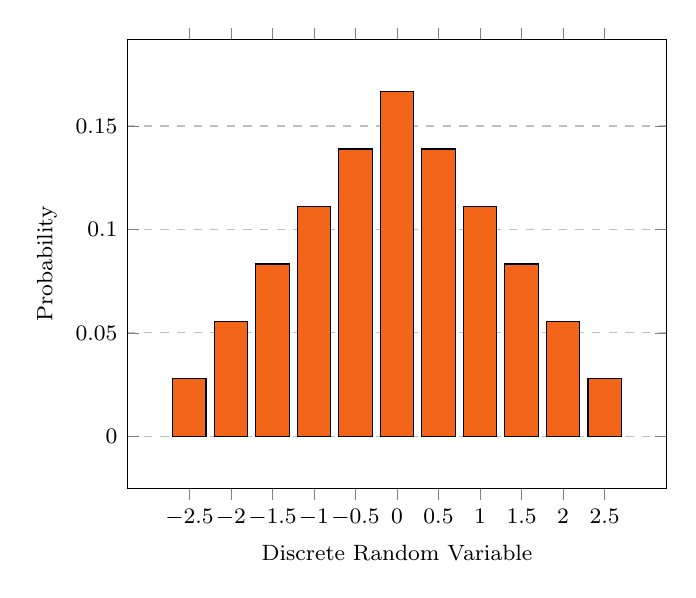
\begin{tikzpicture}
    \begin{axis}[
        ybar,
        bar width=12pt,
        ymin=0,
        xlabel={Discrete Random Variable},
        ylabel={Probability},
        xtick={-2.5,-2,...,2.5},
        xticklabel style={font=\footnotesize},
        yticklabel style={font=\footnotesize, /pgf/number format/fixed},
        xlabel style={font=\footnotesize},
        ylabel style={font=\footnotesize},
        xticklabel style={/pgf/number format/fixed},
        enlargelimits=0.15,
        ymajorgrids=true,
        grid style=dashed
    ]
    \addplot[fill={rgb,255:red,243;green,102;blue,25}] coordinates {
        (-2.5, 0.0278)
        (-2.0, 0.0556)
        (-1.5, 0.0833)
        (-1.0, 0.1111)
        (-0.5, 0.1389)
        (0.0, 0.1667)
        (0.5, 0.1389)
        (1.0, 0.1111)
        (1.5, 0.0833)
        (2.0, 0.0556)
        (2.5, 0.0278)
    };
    \end{axis}
\end{tikzpicture}
\caption{\label{fig:law_large_numbers_1}Probability mass function of the discrete random variable $\frac{X_1 + X_2 }{2} - \mathbb{E}(X)$.}
\end{figure}

Now let's consider a random sample of size ten. In Figure \ref{fig:law_large_numbers_2} is depicted the probability mass function of the discrete random variable $\frac{X_1 + X_2 + \ldots +  X_{10}}{10} - E(X): \Omega \times \ldots \times \Omega \rightarrow \mathbb{R}$. The probability $P(  |\frac{X_1 + X_2 + \ldots +  X_{10}}{10} - E(X)| < 1 )$ is $0.973$.

\begin{figure}[t]
\centering
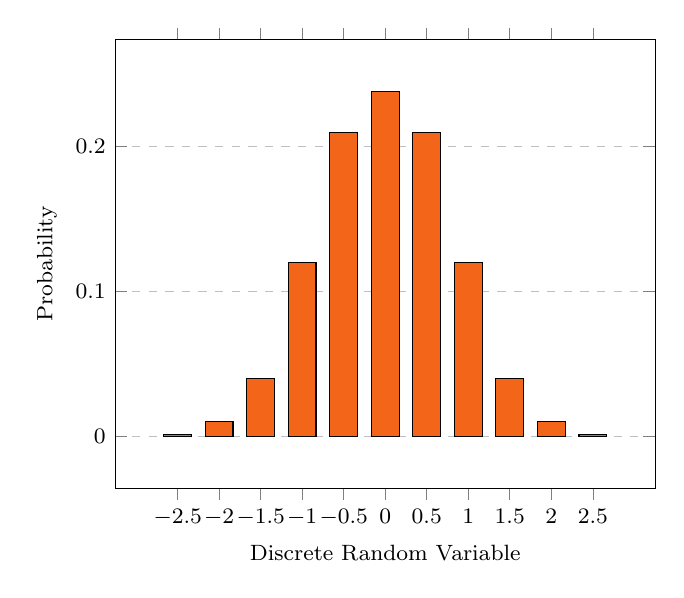
\begin{tikzpicture}
    \begin{axis}[
        ybar,
        bar width=10pt,
        ymin=0,
        xlabel={Discrete Random Variable},
        ylabel={Probability},
        xtick={-2.5,-2,-1.5,-1,-0.5,0,0.5,1,1.5,2,2.5},
        xticklabel style={font=\footnotesize},
        yticklabel style={font=\footnotesize},
        xlabel style={font=\footnotesize},
        ylabel style={font=\footnotesize},
        xticklabel style={/pgf/number format/fixed},
        enlargelimits=0.15,
        ymajorgrids=true,
        grid style=dashed
    ]
    \addplot[fill={rgb,255:red,243;green,102;blue,25}] coordinates {
        (-2.5, 0.0010)
        (-2.0, 0.0100)
        (-1.5, 0.0400)
        (-1.0, 0.1200)
        (-0.5, 0.2100)
        (0.0, 0.2380)
        (0.5, 0.2100)
        (1.0, 0.1200)
        (1.5, 0.0400)
        (2.0, 0.0100)
        (2.5, 0.0010)
    };
    \end{axis}
\end{tikzpicture}
\caption{\label{fig:law_large_numbers_2}Probability mass function of the discrete random variable $\frac{X_1 + X_2 + \ldots +  X_{10}}{10} - E(X)$.}
\end{figure}

\end{example}

It is important to clarify that the law of large numbers refers to the sample mean, that is $\frac {1}{n} \sum_{i=1}^{n} X_{i}$, and it is not necesarily true for other formulas, like for example, the deviation from the theoretical expected value $\sum_{i=1}^{n} X_{i} - n \times E(X)$ which not only it does not converge, but inscreases in absolute value as $n$ increases (see Example \ref{ex:gambler's_fallacy}).

\begin{example}
\label{ex:gambler's_fallacy}
If we toss a fair coin, the probability that the outcome will be head is equal to $1/2$. According to the law of large numbers, the proportion of heads in a large number of coin tosses will be close to $1/2$. However, the difference between the number of heads and tails will not be close to zero. In fact, the larger the number of coin tosses, the larger will be this difference. This is a highly conterintuitive fact, since most of the people think that the more we toss the coin, the closer will be the number of heads to the number of tails, which is not true.
\end{example}

% Central Limit Theorem

\subsection{Central Limit Theorem}

Let $X_1, \ldots, X_n$ be a sample of $n$ independent and identically distributed discrete random variables with mean $\mu$ and variance $\sigma^2$. As we saw in the previous section, the law of large numbers states that the sample average $\overline {X}_n$ converges in probability to $\mu$ as $n$ increases. The central limit theorem states that the distribution of the difference between the sample average $\overline {X}_n$ and the population mean $\mu$, when multiplied by the factor $\sqrt {n}$ approximates to the normal distribution with mean $0$ and variance $\sigma^2 / n$. The theorem is true regardless of the shape of the original random vairables.

\begin{theorem}[Central Limit Theorem]
\label{th:central_limit_theorem_pdf}\index{Central limit theorem}
Let $X_{1}, \ldots, X_{n}$ be a random sample of size $n$ from a distribution with mean $\mu$ and finite variance $\sigma^{2}$. Define the standardized sum as
\[
Z_n = \frac{\overline{X}_{n}-\mu}{\sigma/\sqrt{n}},
\]
where $\overline{X}_{n} = \frac{1}{n} \sum_{i=1}^{n} X_i$ is the sample mean. Then, as $n \rightarrow \infty$, the probability density function of $Z_n$ converges to the probability density function of the standard normal distribution $\phi(x)$, that is,
\[
\lim_{n \rightarrow \infty} f_{Z_n}(x) = \phi(x),
\]
where $f_{Z_n}(x)$ is the probability density function of $Z_n$, and $\phi(x)$ is the probability density function of the standard normal distribution, given by
\[
\phi(x) = \frac{1}{\sqrt{2\pi}} \exp\left(-\frac{x^2}{2}\right).
\]
\end{theorem}
\begin{proof}
Let $X_{1}, \ldots, X_{n}$ be independent and identically distributed (i.i.d.) discrete random variables with mean $\mu$ and finite variance $\sigma^2$. Define the sample mean as
\[
\overline{X}_n = \frac{1}{n} \sum_{i=1}^{n} X_i.
\]
We are interested in the distribution of the standardized variable
\[
Z_n = \frac{\overline{X}_n - \mu}{\sigma / \sqrt{n}}.
\]

First, consider the sum of the $X_i$'s, which we write as
\[
S_n = \sum_{i=1}^{n} X_i.
\]
The sample mean can then be written as
\[
\overline{X}_n = \frac{S_n}{n}.
\]
Thus, the standardized variable $Z_n$ becomes
\[
Z_n = \frac{S_n - n\mu}{\sigma\sqrt{n}}.
\]

To analyze the behavior of $Z_n$ as $n \to \infty$, we consider the sum $S_n = \sum_{i=1}^{n} X_i$. According to the Law of Large Numbers, $S_n/n$ converges to $\mu$, and hence $Z_n$ should converge to a normal distribution due to the nature of sums of independent discrete random variables.

For large $n$, $Z_n$ can be approximated by considering the Taylor expansion of the exponential function. Since the $X_i$'s are i.i.d., the distribution of $S_n$ can be approximated by a normal distribution with mean $n\mu$ and variance $n\sigma^2$. The key idea is that as $n$ increases, the distribution of $Z_n$ approaches a normal distribution because the sum of i.i.d. discrete random variables tends to be normally distributed by the Central Limit Theorem.

Let us consider the moment generating function (MGF) of $Z_n$. The MGF of $Z_n$ is given by:
\[
M_{Z_n}(t) = \mathbb{E}\left[\exp\left(t Z_n\right)\right] = \mathbb{E}\left[\exp\left(t \frac{S_n - n\mu}{\sigma\sqrt{n}}\right)\right].
\]
For large $n$, by the Central Limit Theorem, the MGF of $Z_n$ approaches that of a standard normal variable $N(0,1)$:
\[
M_{Z_n}(t) \approx \exp\left(\frac{t^2}{2}\right),
\]
which implies that $Z_n$ converges in distribution to $N(0,1)$ as $n \to \infty$.

Since $Z_n$ converges in distribution to $N(0,1)$, the probability density function of $Z_n$, denoted by $f_{Z_n}(x)$, must converge to the probability density function of a standard normal distribution $\phi(x)$, given by:
\[
\phi(x) = \frac{1}{\sqrt{2\pi}} \exp\left(-\frac{x^2}{2}\right).
\]
Thus, we have
\[
\lim_{n \rightarrow \infty} f_{Z_n}(x) = \phi(x).
\]

Therefore, as $n \to \infty$, the distribution of the standardized sum $Z_n$ approaches the standard normal distribution, completing the proof.
\end{proof}

The Central Limit Theorem is a fundamental concept in probability theory used in statistical analysis and inference. It allows us to compute the probability that the sample average is close to the distribution mean. It is important to recall the conditons for the central limit theorem to be true: the samples must be independent and identically distributed, the original distribution has to have a finite variance, and the sample size must be sufficiently large.

\begin{example}
Suppose a factory produces light bulbs, and the lifespan of each light bulb is a discrete random variable with a mean of $\mu = 1000$ hours and a standard deviation of $\sigma = 50$ hours. The factory tests a random sample of $n = 36$ light bulbs to estimate the average lifespan of the bulbs produced in a particular batch. What is the probability that the sample mean lifespan of these 36 bulbs is between 990 and 1010 hours?

We can apply the Central Limit Theorem to solve this problem because we are dealing with the sample mean of a large number of independent, identically distributed discrete random variables (lifespans of light bulbs). First, define the sample mean $\overline{X}_n$ as:
\[
\overline{X}_n = \frac{1}{n} \sum_{i=1}^{n} X_i,
\]
where $X_i$ represents the lifespan of the $i$-th light bulb in the sample, and $n = 36$ is the sample size.

By the Central Limit Theorem, for sufficiently large $n$, the distribution of the sample mean $\overline{X}_n$ approaches a normal distribution with mean $\mu$ and standard deviation $\sigma/\sqrt{n}$:
\[
\overline{X}_n \sim N\left(\mu, \frac{\sigma}{\sqrt{n}}\right) = N\left(1000, \frac{50}{\sqrt{36}}\right) = N\left(1000, \frac{50}{6}\right) = N\left(1000, 8.33\right).
\]

Next, we calculate the z-scores corresponding to 990 hours and 1010 hours using the formula:
\[
z = \frac{X - \mu}{\sigma/\sqrt{n}},
\]
where $X$ is the value for which we want to find the z-score.

For $X = 990$:
\[
z_{990} = \frac{990 - 1000}{8.33} \approx \frac{-10}{8.33} \approx -1.20.
\]

For $X = 1010$:
\[
z_{1010} = \frac{1010 - 1000}{8.33} \approx \frac{10}{8.33} \approx 1.20.
\]

Now, we use the standard normal distribution table (or a calculator) to find the probabilities corresponding to these z-scores:
\[
P(z_{990} \leq Z \leq z_{1010}) = P(-1.20 \leq Z \leq 1.20).
\]

From the standard normal distribution table:
\[
P(Z \leq 1.20) \approx 0.8849,
\]
\[
P(Z \leq -1.20) \approx 0.1151.
\]

Thus, the probability that the sample mean lifespan of the 36 light bulbs is between 990 and 1010 hours is:
\[
P(990 \leq \overline{X}_n \leq 1010) = P(-1.20 \leq Z \leq 1.20) = 0.8849 - 0.1151 = 0.7698.
\]

The probability that the sample mean lifespan of the 36 light bulbs falls between 990 and 1010 hours is approximately 76.98\%. This result demonstrates how the Central Limit Theorem allows us to use the normal distribution to approximate the sampling distribution of the sample mean, even when the original data is not normally distributed, as long as the sample size is sufficiently large.
\end{example}

%
% Section: References
%
\section*{References}

\cite{degroot1986probability} is a widely respected textbook in the fields of statistics and probability theory. First published in 1975, this book is known for its clear exposition of the fundamental concepts of probability and statistics, making it suitable for both beginners and those with some background in the subject. The book's approach balances theory and application, making it useful both for learning theoretical underpinnings and for applying probability and statistics to real-world problems.

\cite{childers2013philosophy} offers a comprehensive introduction to the foundational aspects of probability, with a focus on the philosophical questions it raises. Childers explores various interpretations of probability, including frequentist, propensity, classical, Bayesian, and objective Bayesian, and presents these complex ideas in a way that is accessible even to those without a strong background in probability or mathematics.

An example of the problems associated with the misinterpretation of expected value is the St. Petersburg Paradox\index{St. Petersburg Paradox}. Introduced by Nicholas Bernoulli in 1713, this paradox involves a gambling game with an infinite expected payoff, yet no reasonable person would pay more than \$25 to play it. Despite being three centuries old, the paradox continues to inspire new arguments and solutions in recent years (see \cite{huang2013three} for a historical review of the main proposed solutions).
